\documentclass[12pt]{article}
\input epsf

\usepackage{fullpage}
\usepackage{multirow}
\usepackage{caption}
\usepackage{graphicx}
\usepackage{subfig}     % Neccessary for subfigures, needs to be installed
\usepackage{hyphenat}
\usepackage{color,fancyvrb}
\usepackage{setspace}
%

\def\beqn{\begin{eqnarray}}
\def\eeqn{\end{eqnarray}}



\textwidth  6.in
\textheight 8.5in
\topmargin 0. in
\oddsidemargin 0in
\evensidemargin 0in
\pagenumbering{arabic}
%
\newcommand{\Thgg}{$\theta_{\gamma^*\gamma}~$}
\newcommand{\Phgg}{$\phi_{\gamma^*\gamma}~$}
\newcommand{\Epg}{$ep~\rightarrow~ep\gamma~$}
\newcommand{\Eppiz}{$ep~\rightarrow~ep\pi^o~$}
\newcommand{\Enpip}{$ep~\rightarrow~en\pi^+~$}
\newcommand{\EppiD}{$ep~\rightarrow~e\pi \Delta~$}
\newcommand{\Epeta}{$ep~\rightarrow~ep\eta~$}
\newcommand{\Epr}{$ep~\rightarrow~ep\rho~$}
\newcommand{\EpX}{$ep~\rightarrow~epX~$}
\newcommand{\EpKY}{$ep~\rightarrow~eKY~$}
\newcommand{\vEpg}{$\vec ep~\rightarrow~ep\gamma~$}
\def\gevc2{(GeV/c)$^2$}
\begin{document}
\pagestyle{plain}
%\indent
%\input{central_introduction.tex}
%\input{central_solenoid.tex}
%\input{central_tracker.tex}
%\input{central_tof.tex}%
%\input{central_ec.tex}%
%\begin{thebibliography}{99}
%% \bibitem{CLAS12G}

\bibitem{BONUS} JLab E03-12, The Structure of the Free Neutron Via Spectator 
Tagging. H. Fenker, C. Keppe, S. Kuhn and W. Melnitchouk spokespersons.  

\bibitem{ZHENG}
X. Zheng {\it et al.},
Phys. Rev. Lett. {\bf 92}, 012004 (2004);
Phys. Rev.  {\bf C70} 065207 (2004).

\bibitem{VIPULI} K.V. Dharmawardane {\it et al.},
Phys.Lett. {\bf B641} 11 (2006).

\bibitem{BONUS12} JLab  E12-06-113, The Structure of the Free Neutron at 
Large x-Bjorken. S. Bueltmann, M. Christy, H. Fenker, K. Griffioen, 
C. Keppel, S. Kuhn, W. Melnitchouk, V. Tvaskis spokespersons.  

\bibitem{EG12} E12-06-109 The Longitudinal Spin Structure of the Nucleon. 
D. Crabb, A. Deur, K. Dharmawardane, T. Forest, K. Griffioen, M. Holtrop, 
S. Kuhn, Y. Prok

\bibitem{KUHL}
S.~Kuhlmann {\em et al.},
Phys. Lett. B {\bf 476}, 291 (2000).

\bibitem{MT}
W.~Melnitchouk and A.~W.~Thomas,
Phys. Lett. B {\bf 377}, 11 (1996).

\bibitem{Leader:2005ci}
  E.~Leader, A.~V.~Sidorov and D.~B.~Stamenov,
  %``Longitudinal polarized parton densities updated,''
  Phys.\ Rev.\ D {\bf 73}, 034023 (2006)
  [arXiv:hep-ph/0512114].
  %%CITATION = HEP-PH 0512114;%%

\bibitem{Dharmawardane:2006zd}
  K.~V.~Dharmawardane, S.~E.~Kuhn, P.~Bosted and Y.~Prok  [the CLAS
                  Collaboration],
  %``Measurement of the $x$- and $Q^2$-Dependence of the Asymmetry $A_1$ on the
  %Nucleon,''
  to be published in Phys. Lett., arXiv:nucl-ex/0605028.
  %%CITATION = NUCL-EX 0605028;%%


 \bibitem{EG1a}
R. Fatemi {\it et~al.} [CLAS Collaboration],
Phys. Rev. Lett. {\bf 91}, 222002 (2003),
J. Yun  {\it et~al.} [CLAS Collaboration],
Phys. Rev. C {\bf 67}, 055204 (2003).

\bibitem{rev_mom}
J.-P. Chen, A. Deur, Z.-E. Meziani, Mod. Phys. Lett. \textbf{A20}, 2745 (2005);
M. Osipenko {\it et al.}, Phys. Rev. D {\bf 71}, 054007 (2005).


\bibitem{Bj}
J. D. Bjorken, Phys. Rev. \textbf{148}, 1467 (1966).

\bibitem{GDH}
S. D. Drell and
A. C. Hearn, Phys. Rev. Lett. \textbf{16}, 908 (1966);
S. Gerasimov, Sov. J. Nucl. Phys. \textbf{2}, 430 (1966).

\bibitem{JiSR}
X. Ji and J. Osborne, J. Phys. {\bf G27} 127 (2001).

\bibitem{HERMES}
HERMES collaboration: A. Airapetian \emph{et al.}, 
Eur. Phys. J. {\bf C26}, 527 (2003).

\bibitem{E143}
E143 collaboration: K. Abe \emph{et al.},
Phys. Rev. Lett. \textbf{78}, 815 (1997); 
K. Abe \emph{et al.}, 
Phys. Rev. D {\bf58}, 112003 (1998).

\bibitem{E155}
P.L. Anthony {\it et al.,} Phys. Lett. {\bf B493}, 19 (2000).

\bibitem{AO}
V. D. Burkert and B. L. Ioffe,
Phys. Lett. \textbf{B296}, 223 (1992);
J. Exp. Theor. Phys. {\bf 78}, 619 (1994).

\bibitem{BT} N. Bianchi and E. Thomas,
Nucl. Phys. Proc. Suppl. \textbf{82}, 256 (2000).

\bibitem{BjHT} 
A. Deur {\em et al.}, Phys. Rev. Lett. {\bf 93} 212001 (2004)

\bibitem{E97110} J.P. Chen, A. Deur and F. Garibaldi, JLab experiment
E97-110

\bibitem{E03006} M. Battaglieri, A. Deur, R. De Vita and M. Ripani,
JLab experiment E03-006

\bibitem{BG}
E.~D.~Bloom and F.~J.~Gilman,
Phys. Rev. Lett. {\bf 16}, 1140 (1970);
Phys. Rev. D {\bf 4}, 2901 (1971).

\bibitem{NIC}
I.~Niculescu {\em et al.},
Phys. Rev. Lett. {\bf 85}, 1182, 1186 (2000).

\bibitem{d2n} M. Amarian {\em et al.}, 
Phys. Rev. Lett. {\bf 92} 022301 (2004)


\bibitem{BOSTED EG1b}P.E. Bosted {\it et al.},
hep-ph/0607283


\bibitem{E01-012} P. Solvigon, Contribution to the proceedings of the First 
Workshop on Quark-Hadron Duality and the Transition to pQCD. A. Fantoni, 
S. Luiti and O. Rondon ed. World Scientific, 2006.


\bibitem{ERIC}
M.~E.~Christy {\em et al.},
E94-110 Collaboration, in preparation.

\bibitem{osipenko} 
M. Osipenko {\em et al.}, Phys. Rev. {\bf D67} 09201 (2003)

\bibitem{noi} 
S. Simula and M. Osipenko, Nucl. Phys. {\bf B675} 289 (2003)

\bibitem{alpha} S. Bethke, $\alpha_S$ 2002 High-Energy Physics Int'l 
Conference in Quantum Chromodynamics, Montpellier (France) (2002)

\bibitem{GDH04} K. Helbing. Talk given at the GDH04 symposium. 
www.physics.odu.edu/GDH2004/Proceedings/Helbing.pdf

\bibitem{SLACGDH} SLAC experiment E159. P. Bosted and D. Crabb spokespersons.
www.slac.stanford.edu/exp/e159/prop.pdf

 
\bibitem{DGP}
A.~de~R\'ujula, H.~Georgi and H.~D.~Politzer,
Ann. Phys. {\bf 103}, 315 (1975).

\bibitem{DUALMODEL}
N.~Isgur, S.~Jeschonnek, W.~Melnitchouk and J.~W.~Van Orden,
Phys. Rev. D {\bf 65}, 054005 (2001).


%\end{thebibliography}
%\end{document}
\title
{
\vspace{-1.4cm}
\begin{flushright}
\normalsize{Draft; source file /u/home/baturin/DocCVS/12gev/TDR/TDR2007/main/detector/central/ctof/ctofmagshield310108.tex}
%\bigskip
%\bigskip
%\bigskip
%\bigskip
%\bigskip
%\bigskip
%\bigskip
%\bigskip
\nopagebreak
\end{flushright}Magnetic shielding for the CLAS12 Central TOF detector.}
\author
{
{}\\
%{}\\
%{}\\
%{}\\
%{}\\
%{}\\
\mbox
{V.Baturin, V.Burkert, D.Carman,} \\
{ L.Elouadrhiri, Ph.Fazilleau, Y.Sharabian, V.Kubarovsky,} \\
{W.Kim, G.S.Mutchler, A.Ni, J.Riso.} \\
{and} \\
{ B.Wieland, T.Madlem}
%{}   \\
%{ }   \\
%{}\\harmful
%{}\\
\mbox
{}\\
%{}\\
%{}\\
%{}\\
{}\\
}
\maketitle


%\begin{flushleft}
%\end{flushleft}


\tableofcontents
\newpage
\listoftables
\newpage
\listoffigures
\newpage
\section{Introduction}

The Central Time Of Flight detector ({\tt CTOF})
 is being designed at JLab with the  ordinary PMTs, coupled
to the scintillators via $\approx1.6m$-long light guides of complex design
\footnote{We  anticipate that  at
final stage of designing   the regular PMTs may be replaced
with fine mesh PMTs with twice shorter light guides. These PMTs
 are insensitive  up to 5000Gs.}.
The PMT layout in the current  {\tt CTOF} design  
is shown in 
%Fig.{\ref{barrel}} and 
Fig.{\ref{barrel2}}.
%%%%%%%%%%%%%%%%%%%%%%%%%%%%%%%%%%%%%%%%%%%%%%%%%%%%%%%%%%%%%%%%%%%%%%%%%%%
%\begin{figure}[htbp]
%\centering
%\includegraphics[width=0.7\textwidth]{CLASTOF.ps}
%\caption{\small{The design of the {\tt CLAS12} central TOF
%detector.}}
%\label{barrel}
%\end{figure}
%%%%%%%%%%%%%%%%%%%%%%%%%%%%%%%%%%%%%%%%%%%%%%%%%%%%%%%%%%%%%%%%%%%%%%%%%%%



%%%%%%%%%%%%%%%%%%%%%%%%%%%%%%%%%%%%%%%%%%%%%%%%%%%%%%%%%%%%%%%%%%%%%%%%%%%
\begin{figure}[htbp]
\centering
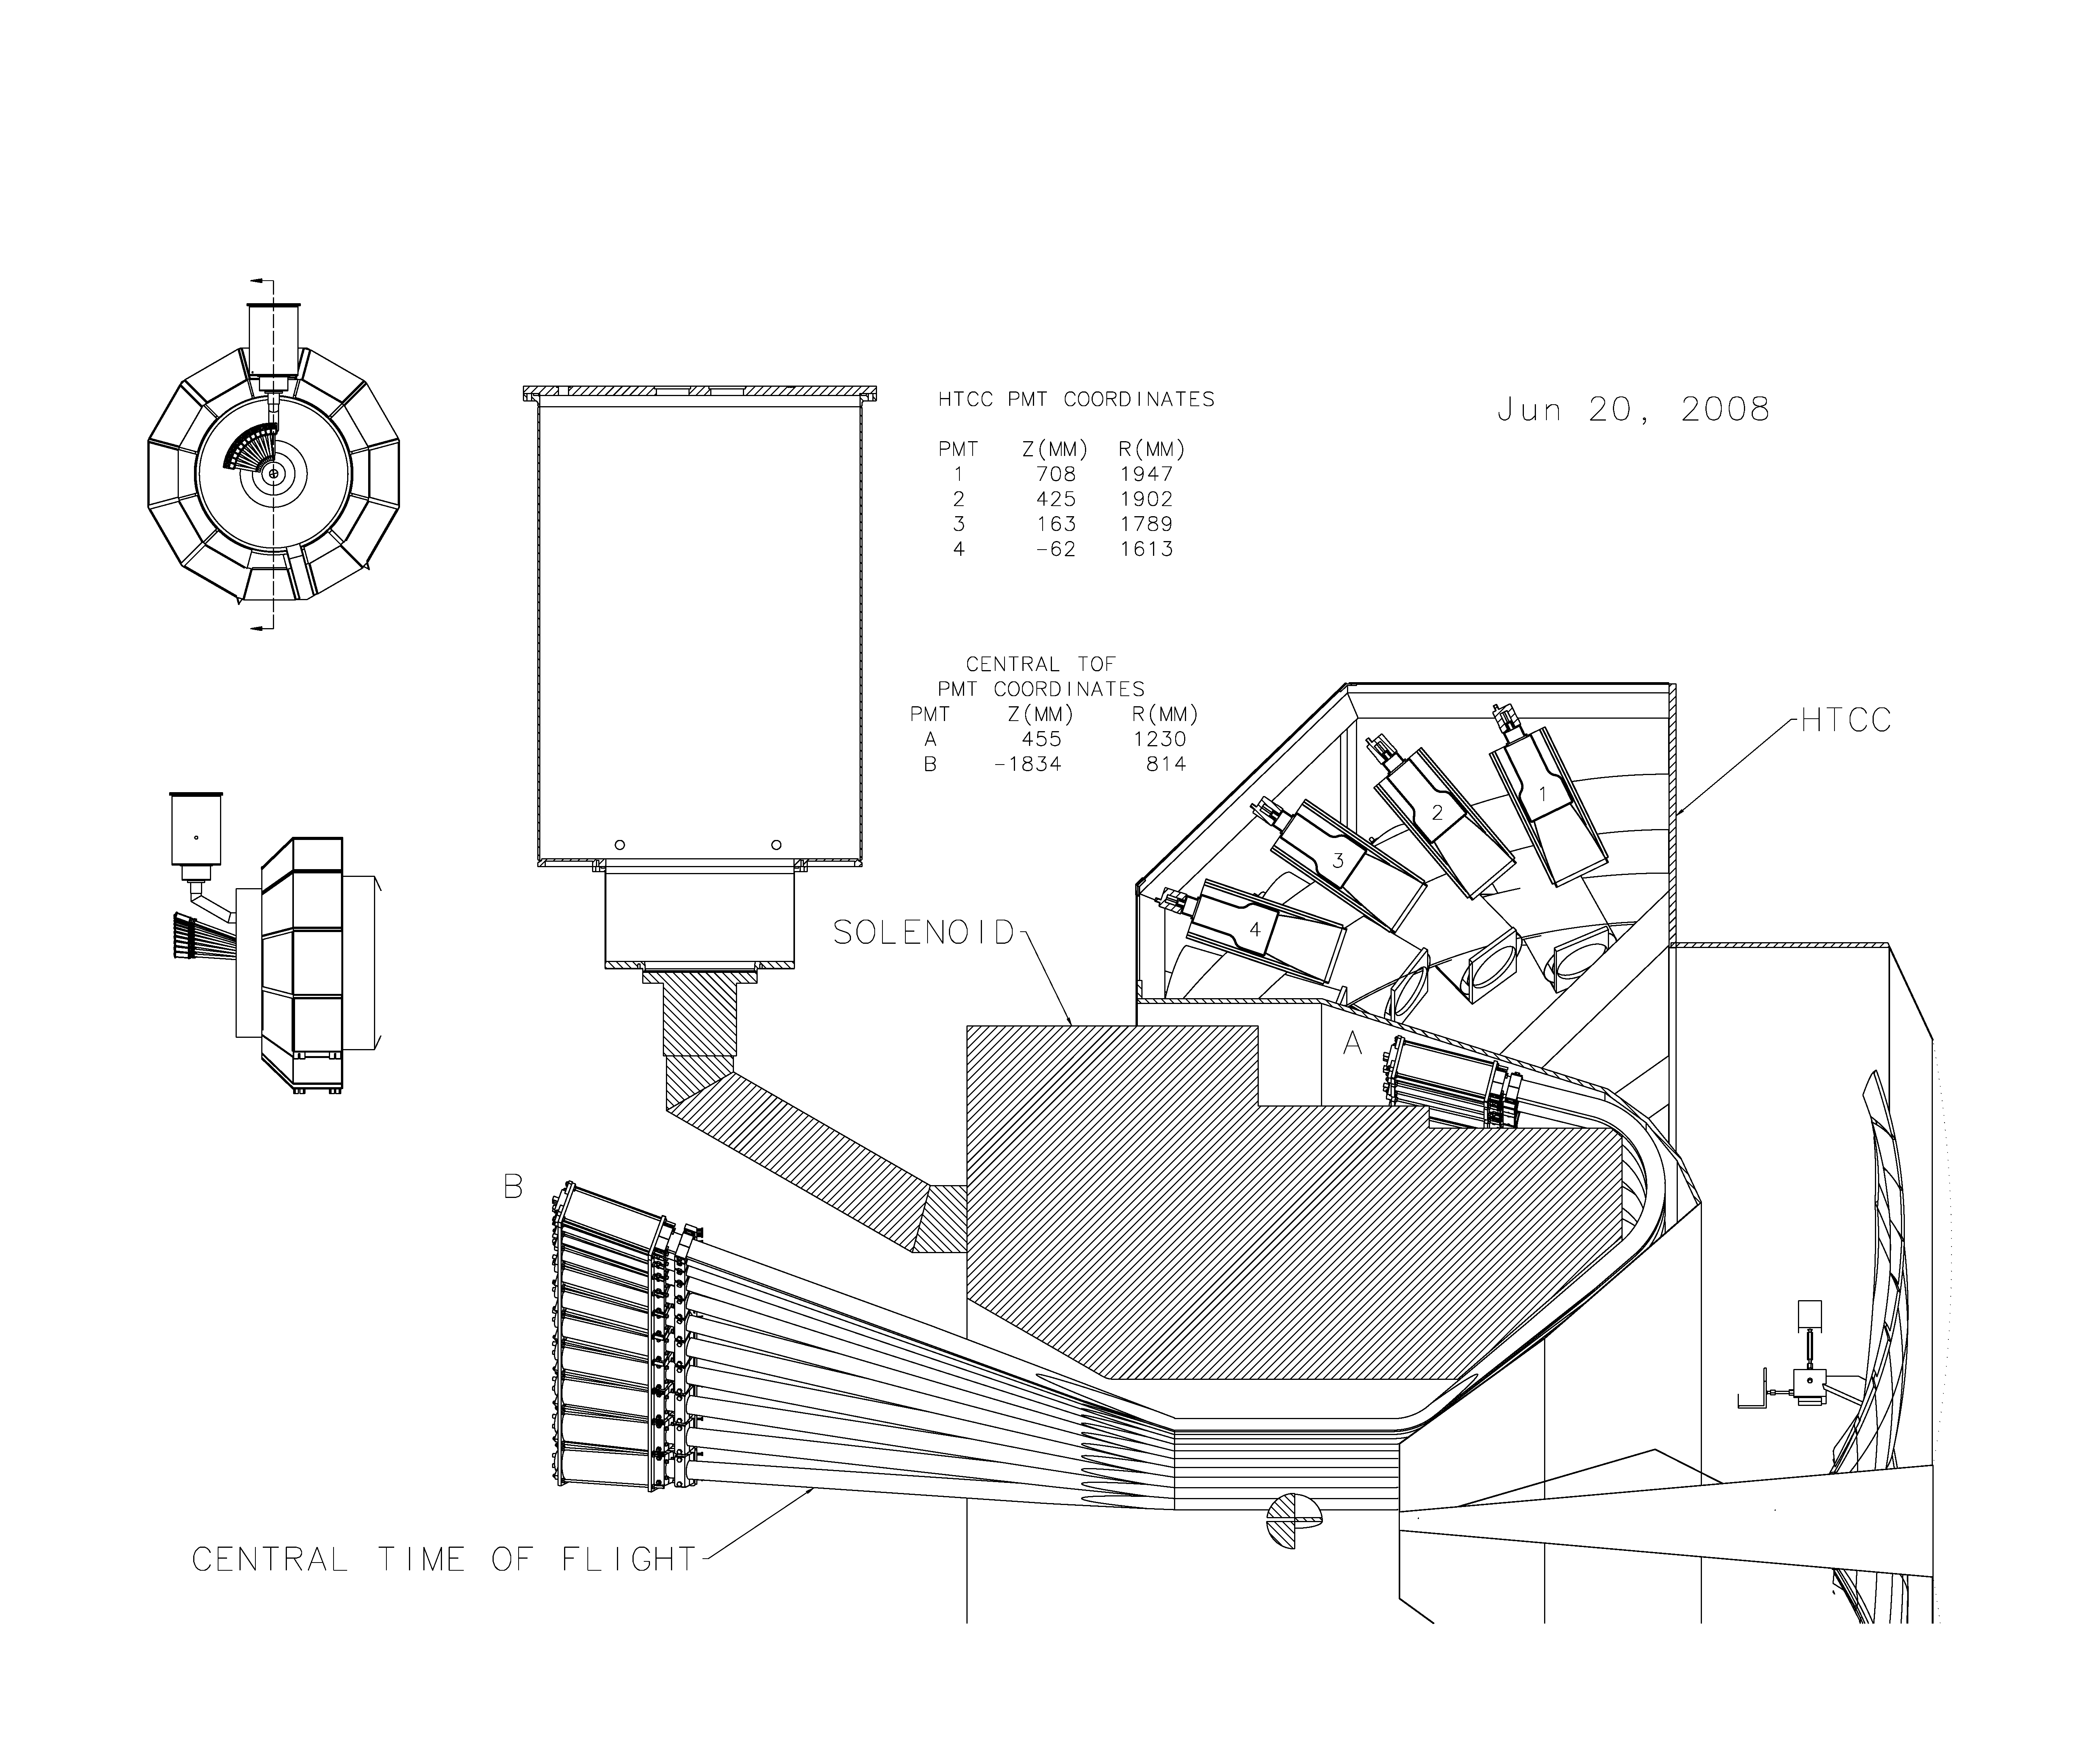
\includegraphics[width=0.8\textwidth]{HTCC_CTOF_STUDY_060507_WRAP.eps}
\caption{\small{The layout of the {\tt CLAS12} central TOF detector.
The solenoid is shown by the hatched area.  The scintillators form a barrel,
66-cm long with an inner radius 24.945~cm.  At the upstream and downstream
ends, 50-mm diameter light guides are included that have a pitch of
20$^\circ$ and 41$^\circ$, respectively.  The 1.4 and  1.6-m long light guides
for conventional upstream and downstream PMTs,  respectively,
may be replaced with $\leq$1-m long light guides to accommodate magnetic-field-immune photo-detectors.}}
\label{barrel2}
\end{figure}
%%%%%%%%%%%%%%%%%%%%%%%%%%%%%%%%%%%%%%%%%%%%%%%%%%%%%%%%%%%%%%%%%%%%%%%%%%%
With this design  we
are aiming for the TOF resolution of $50-60ps$ using a double-sided readout
with conventional PMTs via very  long light guides ($\leq 1.6$~m), delivering
light to an area outside of the central solenoid where the associated
magnetic fields are low. The corresponding field map is shown in  Fig.~\ref{fig:mmap1}.


Our basic  PMT is $51mm$ R2083 from Hamamatsu.
As most of timing PMTs it has a spherical photo cathode $46mm$ in diametr.
Such shape is helpful to  equalize travel  distances of primary photo electrons. 
R2083 has a  shortest rize time 0.7ns  and  TTS of 370ps. 

Due to a spherical shape of the photo cathode    
 axial  fields at the photo cathode 
are not  possible. Therefore, PMTs with spherical photo cathode
are more  sensible to fringe  magnetic fields.

The design of R2083  is similar   to XP4312, which also has a spherical 
photo cathode, but is  $76mm$ in diameter. Thus, it is more sensitive to magnetic 
fields. This PMT  was sorrowsly studied in 1993 by J.Flint
and E.Smith as a candidate to the CLAS TOF detectors. It was shown that XP4312    
manifests  an  additional time smearing of $\leq30ps$  at magnetic fields 
of  $0.2-0.4G$\footnote{See a corresponding fieldmap in Fig.13 of  CLAS Note 94-008}.
Since our PMT is similar in design we can admit these values as  maximum fields 
at the photo cathode of R2083. However, we aim to lower fields of $\leq0.1G$
for redundancy.
%It will be clear from the further consideration  that in the 3 layer shielding with a thin
%high permeability inner layer, the field at the photo cathode may be reduced to practical zero.

%%%%%fig#3%%%%%%%%%%%%%%%%%%%%%%%%%%%%%%%%%%%%%%%%%%%%%%%%%%%%%%%%%%%%%%%%
\begin{figure}[htbp]
\centering
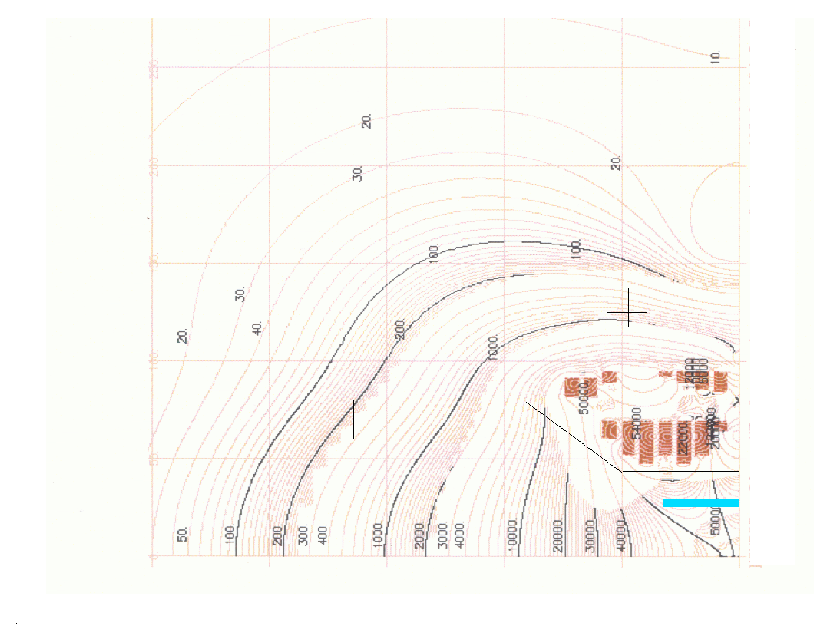
\includegraphics[width=0.9\textwidth]{mmap1.eps}
\caption{\small{Location of R2083 PMTs (cross-hairs) in relation to a
magnetic field map of the central {\tt CLAS12} solenoid.}}
\label{fig:mmap1}
\end{figure}
%%%%%%%%%%%%%%%%%%%%%%%%%%%%%%%%%%%%%%%%%%%%%%%%%%%%%%%%%%%%%%%%%%%%%%%

As one can see from the field map in Fig.~\ref{fig:mmap1}
at the nominal length of upstream/downstream light guides, 1.4m and 1.6m respectively,
 the R2083 PMTs  require a robust magnetic shield against
of $\leq 500$G and $\leq 250$G, respectively.
 For redundancy we double the  fields to tolerate.
The   optional metal channel PMTs H8500  may operate at 200G  
without magnetic shielding.
However, with a powerful enough  shielding, both kinds of 
PMTs could operate at significantly
higher field. In such a case a  shorter light guides may  be used,
that  improves  the  time resolution.
%  $\approx 30/300~mT$ respectively is  required.
%However, we anticipate that  at
% the final stage of designing  the regular PMTs may be replaced
%with fine mesh PMTs, which are insensitive to magnetic fields up to 700mT.
%  Due to their  different sense areas($S_a$) and
%tolerated magnetic fields $(B_m)$ the corresponding
%light guides has various  transmission lengths($L_t$) and diameters.
%The time being we consider %, as the most realistic candidates,
%the following PMTs\footnote{Unfortunately, recently
% Hamamatsu has discontinued   the most appropriate
%fine mesh PMT R6504 with the photo cathode diameter $51mm$}:
%However, the more efficient is the shield
%the shorter may be light guides, thus the better may be  the time resolution.

%The main  goal of this note is to
% estimate  a  possible shield's   dimensions and  tolerated fields
%using  simple methods suggested by different manufacturers of magnetic shields.
%  Then we
%implicates


In this note we report on our $R\&D$ for the magnetic shieldings
%The main goal of this note is to formulate a research plan
%for  the   
via Final Element Analythis and shield   simulation  in the
homogeneous fringe  magnetic fields.
With   the  results of FEA  calculations we have  designed magnetic shields 
for R2083 and H8500 PMTs.
We plan to  determine the maximum tolerated  fields for thus designed shields
 with 5T magnet and  optimize  the length of light guides for  a 
 better time resolution.
%The most important parameter of the magnetic shield is its maximum  diameter $D_{sm}$.
Under the current design of the CTOF, showm in Fig.\ref{barrel2},
both the downstream
and upstream PMTs are arranged in a circular patterns with the 
corresponding light guides. 
Such design constrains the 
radial coordinates $r_{50}$  of 50 adjacent PMT shields. Thus,  the most important parameter of the shield, its 
diameter $D_{sm}$,  is also constarined\footnote{ To avoid this constraine a more complex design with a  radial 
stagger may be used at the upstrem side, only.}:

\begin{equation}
%D_{sm}=2\frac{r_{50}}{(ctg(3.6^o)-1)} =134.277\times r_{50}.
D_{sm}=2\frac{r_{50}}{sin(3.6^o)} =134.27\times r_{50}.
\label{eq776}
\end{equation}
The relevant characteristics of PMTs are listed below:
\begin{center}
\begin{tabular}{|c|c|c|c|c|c|c|c|c|c|}  \hline
PMT         &$D_{pm}$& $S_a$  & $L_{m}$  &$B_{t}$  & $M$       &$r_{50}$&$D_{sm}$&$L_{LG}$& $B_{o}$   \\
            &$mm$     & $mm^2$ & $mm$     &$G$     & $Kg$      & $mm$   &        &  mm    & $G$     \\ \hline
%
%%%R2083-u   &54       &1662    &120       &0.1      & $\approx5$    & 826    & 110.9  & 1580  &          \\
%
R2083-u     &54       &1662    &120       &0.1      & $\approx10$    & 826    &  86  & 1400   & $\leq250$      \\
R2083-d     &-        &  -     & -        &  -      & $5-10$    & 1090   & $146.4$  & 1600   & $\leq500$     \\ \hline
H8500-u     &72       &2400    &15        &$\leq200$  &$\approx10$&  596   &  80.1  & 945    & 2000     \\
H8500-d     & -       &  -     & -        &  -       &$\approx10$& 890    & 119.5  & 945    & 3000     \\ \hline
\end{tabular}
\end{center}
where
$D_{pm}$ is the nominal  diameter of PMT,
$S_a$ - PMT sensitive area,
$L_{m}$ - maximum length to protect against the magnetic field,
$B_{t}$ - maximum tolerated field by ``naked'' PMT,
$M$       - expected  shielding mass,
$r_{50}$  - radial coordinate according to the current design,
$D_{sm}$  - maximum possible diameter of PMT shield via  Eq.\ref{eq776},
$L_{LG}$  - shortest possible light guide length in current design,
$B_{o}$   - magnetic field at the PMT location at specified light guide length.


According to this table the upstream R2083 shield has to withstand against of $\leq 500G$
provided the light guide length is $1400mm$, only\footnote{For ordinary PMTs we dowble the
tolarating field, for redundancy}. 
In this case the diameter of the magnetic shield has to be below $86mm$.
The downstream R2083 meets a significantly higher nonuniform  magnetic  field.
Provided the  downstream light guide length is 1600mm long the maximum field would
be $\leq 1000G$ and the magnetic shield diameter may be maximum  $146mm$ in this case.

Most likely  R2083 PMTs will be used in the assembly H2431, enclosed into
the $\mu$-metal shielding $0.8mm$ thick, $60mm$ in external diameter and $200mm$ long.
We also  plan to ask Hamamatsu to change the  H2431 design  in order to arrange a
overhung of $30-60mm$ from  the photo cathode side.
It is required for a  more efficient shielding\footnote{The internal field 
drops significantly at the depth of one radius of the shield.}.

%\verb|http://www.mushield.com/design-guide.shtm|

\section{ Principles of shield performance and design.}


Two   kinds of PMT shielding are possible: passive and active shielding.
Active shielding makes use of  magnetic fields produced by a  solenoid  around a PMT to cancel the
internal  field. We do not plan to use active shielding
 because, firstly,  in our case the  interfering  fringe  filed
is  not solenoid-al, secondly,  such shield  will be  more complex and more costly, thirdly, it may be a source of
additional electroni noise.

In a passive shielding  the diamagnetic
of superconducting cylinder could be   used to block the magnetic field  inside the cylinder.
Such  kind of shielding looks very complex and expensive, as well, since it requires cryogenics.

Therefore, we plan to study the  traditional approach  based on the  properties of
 ferromagnetic cylinders.
In such shielding magnetic field lines are concentrated in the bulk of a
ferromagnetic, reducing the fringing fields inside the cylinder.
 However, the efficiency  of such shield in high magnetic fields is limited by the
 maximum magnetic flux density, which is possible to create inside  ferro magnetics, i.e. the saturating field,
which is the most important parameter affecting shiled effectiveness.


%
%Unfortunately, the ferromagnetic shield around PMTs
%need holes in both ends.
%These holes allow the shield to be slid onto the PMT,
%Active shielding makes use of the magnetic field
%produced by a  coil to cancel the
%fringing magnetic field in the PMT's area.
%Active shielding may be  relatively light weight,
% compared to ferromagnetic shielding.
%


%\subsection{Ferromagnetic shielding.}
\subsection{Qualitative consideration of shield performance.}
Let's consider a simplified  model for a PMT  magnetic shield in axial field,
i.e. a ferromagnetic ($\mu>>1$)
cylinder of outer/inner  diameters $D_+/D_-$ , thickness
$t=\frac{1}{2}(D_+-D_-)$ and finite length $L\approx 4D_+$, which is
 placed into a uniform axial  field $B_o$. Assume that the last  is created
 inside an infinitely long  solenoid of inner diameter  $2D_+$.
The conservation of the magnetic flux in such system implicates:
 \begin{equation}
4B_o \pi D_+^2 \approx 4B_{in} \pi D_+^2 + (B_m-B_{in}) \pi (D_+^2-D_-^2),
\label{eq004}
\end{equation}
where  $B_m$ is the  field in the ferromagnetic media, $B_{in}$ - the field  inside  the shielding cylinder.
Neglecting $B_{in}$ compared $B_o$ one can relate   the field in the media, $B_m$, to the field inside the shielding, $B_{in}$,
as follows:
 \begin{equation}
B_m  \approx B_0\frac{D+}{t}=\mu B_{in}~~~;~~~B_{in}= B_0\frac{D+}{t\mu},
\label{eq003}
\end{equation}
where the permeability $\mu$  has to be determined  from the ferromagnetic  magnetization curve $B(H)$ at
the  magnetic flux density  $B_m$. 
These formulas  are  in agreement to the practical  formulas  recommended by
numerous manufacturers of magnetic shields.

%\paragraph{Practical formulas.}
The problem of the  infinite  hollow ferromagnetic cylinders in the uniform
transverse magnetic fields has been  solved analytically\footnote{See the  Gluex-doc-843 Jul-17 by E.Smith}, as well as the
 problem  for ellipsoids in axial fields.  Therefore,  the following formulas
\footnote{Recommended by  the Magnetic Shield
 Corporation.
{\verb |http://www.magnetic-shield.com/dynamics/works.html}}
 are available for estimating  the magnetic shield parameters:
\begin{equation}
S=\frac{B_o}{B_{in}}\approx \mu({B_m})\frac{t}{D_+}~~~;~~~B_m\approx B_o\frac{D_+}{0.8t}~~~;~~~t\approx B_o\frac{D_+}{0.8B_m}
\label{eq000}
\end{equation}
where $S$ stands for the shielding factor of a cylinder,
$\mu(B_m)$ - the permeability in function
   on the field in the shielding material $B_m$
$B_o$ - the external  field, $B_{in}$ - the
 field inside ferromagnetic,
$t$ - the thickness of a shielding material and
$D_+$ - the external diameter of the cylinder.

For a multilayer shielding of $n$ coaxial cylinders, separated by $\approx 1mm$ by radius,
the resulting shielding factor is:
%
\begin{equation}
S=S_1 \times S_2 \times...\times S_n
\label{eq777}
\end{equation}
%
where $S_i,i=1,...,n$ are shielding factors for
$i$-cylinder,  estimated via Eq.\ref{eq000}.

Although the above formulas are recommended  for rough estimations
in perpendicular fields they may be used for axial fields, provided the
cylinder lengths exceeds  four  diameters.

%Hence,  our shielding  will be composed of 2-3  coaxial
%cylinders,  fabricated from different  ferromagnetic  materials.




\subsection{Ferromagnetic materials}
Available ferromagnetic shielding materials come in two types: those with higher saturation and
those with higher permeability.
%, in other words,
%there is always trade-off.
High permeability materials are useful  in small  fields.
Therefore, to ``wrap '' PMTs  high permeability materials has been  used, such as  Co-Netic,
which contains 80.6\% Ni and 14\% Fe and is in the same family metallurgically as Mu-metal. 
%Conetic may be  used for the inner  shield layer around PMTs.
 
In high fields  the  materials with high saturation should be used
since a low saturation material would need to be excessively thick.
The   silicon steel (2.25\% Si, 0.40\% Al, balance Fe) may be implemented as 
external shielding. It has been  widely used  in  industry for relays and motors.
%specifically Allegheny Ludlum Relay Steel #5.
%The composition of silicon steel is 2.25\% Si, 0.40\% Al, balance Fe
It  is easy to form and  has moderately high saturation  $1.56/1.96T$
\footnote{For a  non-oriented/oriented grain makes, respectively}.
The more advanced and expensive  Netic alloy saturates at $2.14T$.

In  moderate fields after the external layer of shielding another  higher permeability material 
Hiperm-49 may be used as intermediate layer.

The magnetisation curves for Netic and Co-netic are given in Fig.\ref{muneco}.
and  in Fig.\ref{hiperm49} for Hiperm-49.


% about 10 cm away from the top flange of the magnet
%in order to catch most of the residual
%leakage field from silicon\u2013iron with
%its high permeability.





%\verb|http://www.mushield.com/design-guide.shtml|

\subsection{Preliminary estimations of shielding factor}

For a qualitative  evaluation of  
shield design  and performance  we  use the  formulas from 
Eq.\ref{eq000} recommended for  perpendicular fields.
%%%%%%%%%%%%%%%%%%%%%%%%%%%%%%%%%%%%%%%%%%%%%%%%%%%%%%%%%%%%%%%%%%%%%%%%%%%
\begin{figure}[htbp]
\centering
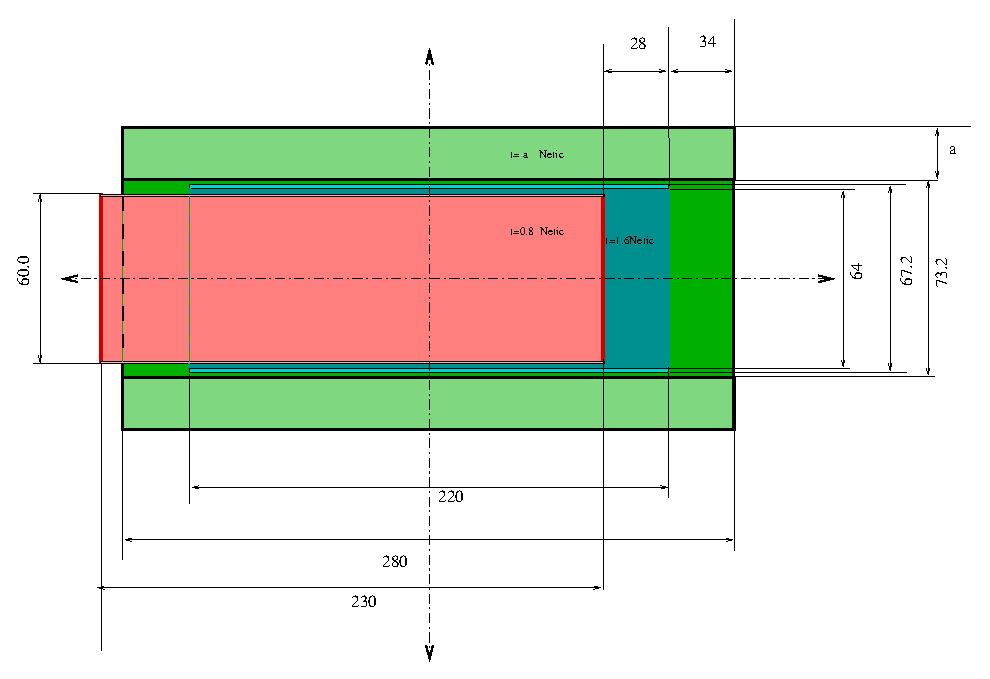
\includegraphics[width=1.0\textwidth]{R2083-3000-ph.eps}
\caption{\small{Pilot design of the R2083 3-layer  magnetic shield. PMT photocathode is supposed to be inside the inner cylinder 
 at the distance of one diameter from the right end.}}
\label{VBT3CY}
\end{figure}
%%%%%%%%%%%%%%%%%%%%%%%%%%%%%%%%%%%%%%%%%%%%%%%%%%%%%%%%%%%%%%%%%%%%%%%%%%%
Refrence   design  for the   R2083 shield is shown in Fig.\ref{VBT3CY}

A detailed FEA calculations 
are  reported in the following  Section-\ref{FEA}.




\paragraph{Shielding factor}
The procedure of estimation is as follows.
Initialy we set the  external magnetic field $B_o$ to be 
tolerated by the shield.
First we estimate the field inside the ferromagnetic $B_m$.
Then  we read the value of $\mu(B_m)$ from the Fig.\ref{muneco}.
Then  we  determine the magnetic field inside the shield, $B_{in}$.
This  procedure will be repeated recursively starting from the outer layer 
with  $B_o=B_{in}$ from the previous step.
The stages  of   such estimations are listed in Table~\ref{ca001}.
In this table  the initial external field was  set 3000G.
Although the field inside the ferromagnetic $(B_m)$ is close to saturation point,
the internal field $(B_{in})$ after the first layer  is only $27.4G$. 
In such low field the permeability of the second layer of the same ferromagnetic 
is 3300, that results in 0.4G field inside the second layer. 
Unexpectedly these rough  estimates  are in qualitative   agreement to the FEA
calculations($0.23G$) performed for us by the Mu-shield company (see Fig.\ref{shieldGrilli}).

\begin{table}[htbp]
\begin{center}
\begin{tabular}{|c|c|c|c|c|c|c|c|c|c|} \hline
Cyl&$B_{o}$ & $D_+$ & $D_-$ & $t$ & $B_m$& $\approx\mu$&$S$      &$B_{in}$     & $Fm$   \\
$n$ &  $G$  & $mm$  & $mm$  & $mm$  & $G$ &           &         &$G$         &     \\ \hline
1 &3000     &  136  &   86  & 25    & 18462&      600  & 110     & 27.4        & Netic   \\ \hline
2 &27.4     &   84  &   80.8& 1.6   & 1797 &     3300  &  63     & 0.4         & Netic   \\ \hline
3 &0.4      &  61.6 &  60   & 0.8   &  11  &    250000 &3300     &$\leq0.001$  & E989-05 \\ \hline
\end{tabular}
\end{center}
\caption{  R2083  shielding  at maximum
field inside  ferromagnetic 18462G.
($n$)~-~layer number starting from the external layer,
($B_{o}$)~-~external field,
($D_+$)~-~external diameter,
($t$)~-~ferromagnetic thickness from   Eq.\ref{eq000},
($B_m$)~-~fields in the ferromagnetic from Eq.\ref{eq000},
($\mu$)~-~permeability  from Fig.\ref{muneco},
($S$)~-~shielding factor,
($B_{in}$)~-~fields inside the shielding external field for a next layer,
($Fm$)~-~ferromagnetic material.
\label{ca001}}
\end{table}
\clearpage

Shield configurations for the H8500 metal channel PMT are listed 
 in Table~\ref{H8500at17600}.
Depending on the maximum  tolerated magnetic flux density by a ferromagnetic,
the external shield diameter may be $128~mm$ or $124~mm$.  
We hope that with FEA simulation it may be further optimized
to the outer diameter $118-120mm$.

%Another possibility of reducing the outer dimension is to use a rectangular pipe
%for shielding.  Magnetic shield companies advertise such  designs. This option has to be studied
%via  FEA calculations, as well.


%3&0.2       &  61.6 &  60  & 0.8   &  11  &     250000&0.006$   &  $\leq\times10^{-3}$ & E989-05 \\ \hline
%%%%%%%%%%%%%%%%%%%%%%%%%%%%%%%%%%%%%%%%%%%%%%%%%%%%%%%%%%%
\begin{table}[htbp]
\begin{center}
\begin{tabular}{|c|c|c|c|c|c|c|c|c|c|} \hline
Cyl&$B_{o}$& $D_+$ & $D_-$ & $t$  & $B_m$  & $\mu$   & $S$    &$B_{in}$         & Fm \\
$n$&$G$    & $mm$  & $mm$  & $mm$ & $G$   &         &        &$G$             &       \\ \hline  
1 &3000    &  128  &  74   & 27   &  17600 &  1000   &  214   &  14             & Netic \\
2 &14      &  74   &  70.8 & 1.6  &  810   &  1800   &  39    & 0.4             & Netic  \\ \hline \hline
1&3000     &   124 &  74   & 25   & 18560  & 600     & 120    & 24.8            & Netic \\ 
2&24.8     & 73.6  &  72   & 0.8  & 2868   & 4500    & 48.6   & 0.5             & Netic \\ \hline
% 2&14     &   -   &   -   &   -  &   -    &  300000 & $10^4$ & 1.5\times10^{-3}& Conetic \\
% 3&0.2    &  61.6 &  60   & 0.8  &   329  &  150000 &$1935$  & 0.1\times10^{-3}& E989-05 \\ \hline
\end{tabular}                                                      
\end{center}
\caption{H8500 shielding  vs  $3000G$  at maximum
fieled inside  ferro-magnetics  $B_m=17600,18500G$.
($n$)~-~layer number starting from the external layer,
($B_{o}$)~-~external field,
($D_+$)~-~external diameter,
($t$)~-~ferromagnetic thickness determined  via   Eq.\ref{eq000}(1-st layer at given $B_m$),
($B_m$)~-~fields in the ferromagnetic determined via  Eq.\ref{eq000}(2-nd layer)
($\mu$)~-~permeability  from Fig.\ref{muneco},
($S$)~-~shielding factor determined via  Eq.\ref{eq000},
($B_{in}$)~-~fields inside the shielding external field for a next layer.
($Fm$)~-~ferromagnetic material. \label{H8500at17600} }
\end{table}
%\clearpage

In Table~\ref{cal2} we study several multy-layer shields for R2083 at 3000, 2000, 1000 and 500G.
As seen form  this table,  the outer cylinder makes the major part of work. 
After it reduce the field up to $10-20G$
the residual field may be easily reduced with a high permeability cylinder such as E989-05, which is
the standard R2083 shielding in the H2431 assembly  from Hamamatsu.
%As can be also seen from this table
Combination with Netic cylinder  115mm(66mm) it may reduce the $3000G$ field to the field $0.004G$ only
This, it is very likely that a two layer shielding $115mm$ in diameter and 1'' thick  may be used in final design.
This means that, since in the last version of CTOF design we have enough space for such shield,
 the light guides may be $110-120cm$ long, only.
Of course  the FEA simulations and optimization  in inhomogeneous magnetic field has to be performed.
%%%%%%%%%%%%%%%%%%%%%%%%%%%%%%
\begin{table}[htbp]
\begin{center}
\begin{tabular}{|r|c|c|c|c|c|c|c|c|c|} \hline
  Shld#&$B_{o}$&$D_+$&$D_-$&$t$   &$B_m$  &$\approx\mu$&$S$   &$B_{in}$         & $Fm$    \\
  -cyl#&  $G$  &$mm$ &$mm$ &$mm$  &$G$   &            &      &$G$            &          \\ \hline 
01-1    &3000 & 126.7 & 72  & 27.3   & 10900 & 4500       & 1200 & 2.5             & Netic    \\ \hline
 2    &2.5  &61.6 &  60 & 0.8  & 140   & 120000     & 1920 &$8\times10^{-4}$  & Conetic \\ \hline
 3    &0.2  &61.6 &  60 & 0.8  & 11    & 250000     & 6000 &$\leq\times10^{-4}$& Conetic \\ \hline\hline  
%02-1    & 3000& 105 & 74  & 15.2 & 17600 & 1000       & 180  & 17              & Netic    \\  \hline
% 2    & 17  & 74  & 71  & 1.6  & 980   & 2000       & 54   & .32             & Netic    \\ \hline \hline 
%03-1    & 3000& 115 & 66  & 24.5 & 17600 & 1000       & 213  & 14              & Netic    \\  \hline
% 2    & 14  & 60  & 58.4& 0.8  & 1312  & 300000     & 4000 & .0035           & E989-05 \\ \hline \hline
03-1    & 3000& 100 &  73.2 & 12.9  &20000 & 250        & 40 &  74           & Netic \\ \hline
%2    & 63.7& 64  & 63.4&  0.8 & 6370  &   80000    &  1000&  0.064          &  Conetic      \\
%2    & 63.7& 64  & 60.8&  1.6 & 3185  &  450000    & 11000&  0.007          &  Conetic      \\ \hline
 2    & 74 & 67.2  &64 & 1.6  &  2760 & 4500       & 134  &  0.5            & Netic       \\ \hline
% 3    & 0.064& 60  &58.4 &0.8    &    6  & 60000     &  800 &      0            & E989-05  \\ \hline
% 3    & 0.7 &  60 &58.4 &  0.8  &  60  & 80000      & 1000 &7\times10^{-4} & E989-05      \\ \hline
 3    & 0.5 &   60 &58.4 &  0.8  &  52  &  200      & 3.3  & 0.15 & Netic      \\ \hline \hline
05-1    & 2000& 92  & 66  & 13.1 & 17600 & 1000       & 142  & 14               & Netic    \\ \hline
% 2    & 14  & 64  & 63.4& 0.8  & 1400  & 350000     & 4375 & .004             & Conetic  \\ \hline
   2    & 14  & 64  & 63.4& 0.8  & 1400  & 3500       & 44   & .4               & Netic    \\ \hline \hline
%%
 06-1    & 1000& 86  & 66  & 9.94 & 10800 & 5000       & 872  & 1.2    & Netic    \\ \hline
    2    & 1.2 & 64  & 63.4& 0.8  &  120  & 100000     & 1250 & 0.001  & E989-05  \\ \hline \hline
 07-1    & 500 & 74.6& 66  & 4.3  & 10800 & 5000       & 250  & 2.0    & Netic    \\ \hline
    2    & 2.0 & 60  & 58.4& 0.8  & 187   & 150000     & 2000 & 0.001  & E989-05  \\ \hline
\end{tabular}
\end{center}
\caption{Estimates of R2083 multilayer  shielding effectiveness at
 external fields  $3000$, $2000$, $1000$, $500~G$.
 $n$
-layer number starting from the external layer,
 $B_{o}$
-external field,
$D_+$
-external diameter,
$t$
-ferromagnetic thickness,
$B_m$
 -fields in the ferromagnetic determined via Eq.\ref{eq000},
$\mu$
-permeability determined via Fig.\ref{muneco},
$S$
-shielding factor  determined via Eq.\ref{eq000} ,
$B_{in}$
-fields inside the shielding.
$Fm$
-ferromagnetic material.
\label{cal2}}
\end{table}
%\clearpage

%Another sample of magnetic shield dynamics  is listed  in Table~\ref{htcc} for the
%HTCC detector. The nominal design includes 3
% layers of ferromagnetic. According to this table 
%fields below  $0.01G$ may be achieved with only two layers of Netic and Conetic.


 
Thus, from this simplifield consideration applicable to  perpendicular fields 
we conclude that our shield have to have  at least three stages.  
In realistic design the length of each cylinders is compatible to its diamter and we expect substantial reduction of shielding factor.
%Therefore, a detailed FEA calculations of several 
%three stage models were performed and we discuss the results in Section-\ref{FEA}. 
In  the following Section-\ref{ednmics}  we study  the electrodynamics of   ferromagnetic cylinders  in axual 
field.  From this consideration  we lern that shilding dynamics  is very different from the transvers case and that 
 longitudinal dimensions are of a crutial importance. 
%In realistic design the length of each cylinders is compatible to its diamter.
Therefore, a detailed FEA calculations of several 
three stage models were performed and we discuss the results in Section-\ref{FEA}.



%\begin{table}[htbp]
%\begin{center}
%\begin{tabular}{|c|c|c|c|c|c|c|c|c|c|} \hline
%Cyl&$B_{o}       $ & $D_+$ &  $D_-$ & $t$     &  $B_m$ & $\approx\mu$ &  $S$  & $B_{in}$          & Comm.    \\
%\# &      $G$     & $mm$  &  $mm$  & $mm$    &   $G$ &              &       & $G$              &          \\ \hline  
%%1& 50             & 164.75& 156.75 &   4     &  2578  &   4500       & 110   &  0.46             & Netic    \\ \hline
%%2& 0.46           & 151.37& 149.77 &  0.4    &  2185  &   400000     & 530   &  0.001            & Conetic  \\
%%3& 0.001          & 144.0 &  142.4 &  0.4    &   3185 &  450000      & 11000 &  0.007            &          \\ \hline
%1& 50              & 161.5 & 158.75 & 3.175   &  3179  &   4500       &  88   &  0.57             & Netic    \\ \hline
%%1& 50             & 161.5 & 158.75 & 3.175   &  3179 &   450000      &8800   &  0.0057           & Conetic  \\ \hline
%2&     0.57        & 153.41& 151.37 &  1.02   &  107.2 &   400        & 2.65  &  0.2              & Netic    \\
%2&     0.57        & 153.41& 151.37 &  0.51   &  214.4 &  120000      & 398   &  0.0014           & Conetic  \\ \hline
%3& 0.2             & 145.2 &  144.0 &  0.51   &   71   &  80000       & 280   &  0.0007           & Conetic  \\ \hline


\end{tabular}                                                      
\end{center}
\caption{HTCC  shield  against of  $50G$. \label{htcc}}
\end{table}


\paragraph{Gradient forces}
In this paragraph we estimate the effect of a 
magnetic field gradients.
Due to a significant non-uniformities  
of magnetic fields in the PMT area,
the magnetic shield anticipates a  force \textbf{F}, caused
 by a gradient of the magnetic field energy density:
\begin{equation}
\textbf{F}=grad_rW(r) = grad_r \int d^3 \textbf{x}
\frac
{ \textbf{B_m}^2({\textbf{x}+\textbf{r}})  }
{ 2\mu_{o}\mu( {\textbf{x}+\textbf{r}}  )  }
\label{eq024}
\end{equation}
where  integration has to be  done
 over   internal coordinates of
ferromagnetic(\textbf{x}),
\textbf{r}- stands for external coordinates
of ferromagnetic shield, $B_m$ - is the magnetic flux density inside the ferromagnetic.

Taking into account  relations from Eq.\ref{eq000},
for  the  upper limit  estimate of
integral Eq.\ref{eq024}    one  can write:
%
\begin{equation}
{F_{max}= \frac{\pi l D^3}{t\mu_{o}\mu_{min}}
B_{o}^{max} ( \frac {dB_o} {dx})_{max}}~~~~~~~~~~~
\label{eq034}
\end{equation}
where $B_o^{max}\approx0.3T$  - is the maximum  possible
external field  in the shield area,
$(\frac{dB_m}{dx})_max\approx0.1T\times
(0.05m)^{-1}=2Tm_^{-1}$
 is the maximum possible gradient of
external field, according to the map field in this area,
$\mu_{min}\approx250$  is the minimum possible permeability
from Table~\ref{cal2},
 $l=0.3m, t=0.025m, D=0.12m$ are the  leng(x)th,  thickness
and the diameter of the ferromagnetic cylinder and
$\mu_o = 4\pi 10^{-7}N·A^{-2}$ is the permeability of vacuum.
Substituting all these numbers into  t Eq.\ref{eq034} we find
%
\begin{equation}
F_{max}= \frac{\pi \cdot 0.3 \cdot m
\cdot (0.12 \cdot m)^3 }{0.025\cdot m \cdot
4 \pi 10^{-7}\cdot N \cdot A^{-2} \cdot 600} \cdot
0.3 \cdot T \cdot 2 \cdot T\cdot m^{-1}= 124.4 \cdot N
\label{eq035}
\end{equation}
%$\mu_o = 4\pi 10^{-7} N·A^{-2}$.
%
Thus,  the maximum possible  force, which
may attract the  ferromagnetic shielding to the solenoid,
does not exceed the   shield  weight.  
We plan  to  address the  ``gradient'' forces in future   FEA simulation.

%<<<<<<< ctofmagshield310108.tex








\section{Electro-dynamics of  ferromagnetic cylinders  in axial field.}

\label{ednmics}

Prior to implementing the  methods of  Final Element Analythis  it would  
be  helpful to consider   the electro-dynamics of ferromagnetic  cylinder in axial fields.

Ferromagnetic properties of materials may be
reproduced assuming that  its  inner space
 is filled with  randomly oriented  current loops,
 responsible for a local  magnetization.
 The external  field  just correlates   
 current loops along its direction.
Due to such correlation inner   fields   
are amplified  by  orders of magnitude.
However,  outside the ferromagnetic the resulting field  
drops, since  the  common   field of   current loops
 outside the ferromagnetic is opposite to the internal field. 
 This  is the basic   mechanism of  magnetic  shielding.

   Effectively, only surface currents protect the inner space of shield, since internal  currents cancel each other in the bulk
of the ferromagnetic.
% thus,  resulting in surface currents, only.
Due to a cylindrical symmetry,  the surface  currents  run in $\phi$-directions,
in which connection the current over the inner surface of the cylinder
will be opposite to that of outer surface one. Therefore, our shielding cylinder  may
be approximated by two  thin coaxial solenoids with opposit currents.
The outer solenoid has the diameter $D_+$, while the inner diameter is
$D_-=D_+-t$, where $t$ is the thickness of the original ferromagnetic cylinder.

  At this  point one may forget about the ferromagnetic 
media.  We  replace it now by a field of current loops  in vacuum.
According  to a  known formula for a
field at the axis $z$  of a  finite  solenoid,
the magnetic field, created by the outer
surface of our cylindrical shield  $B_+(z)$,  yields:
%
\begin{equation}
 B_{+}(z)=+\mu_o j_s(Cos~\alpha^+(z)-Cos~\beta^+(z)~)
\label{eq31}
\end{equation}
%
where $j_s$ is the absolute value of surface current density,
 $\alpha_^+(z)$ and $\beta_^+(z)$
are  the two  angles between  $z$-axis and two  vectors ,
from  the  point $z$ to the corresponding butts  of  a  cylinder.

Due to  opposite direction of  the inner 
currents the corresponding field is opposite to that of the  external cylinder:
%
\begin{equation}
%B_-=-\mu_o j_s \frac{L}{\sqrt{L^2+D_-^2}}
B_-(z)=-\mu_o j_s(Cos~\alpha^-(z) - Cos~\beta^-(z)~)
\label{eq32}
\end{equation}
%
Thus, the resulting vacuum field inside the   shield $B_{in}$ , may  be evaluated as
%
\begin{equation}
%B_{in}(z)=B_o + B_+ - B_-\approx B_o-\mu_o j_s \frac{t}{L}
B_{in}-B_o = B_+ - B_-
\approx - \mu_o j_s
\small{(Sin(\frac{\alpha^++\alpha^-}{2})(\alpha^+-\alpha^-)
-Sin(\frac{\beta^++\beta^-}{2})(\beta^+-\beta^-))}
\label{eq1}
\end{equation}
%
%where  factor
%$g(z)\approx 2(Sin^2(\alpha_1)Cos(\alpha_1)-Sin^2(\alpha_2)Cos(\alpha_2))$%
%$g(z)\approx
% Sin(\frac{\alpha^+ + \alpha^-}{2})(\alpha^+-\alpha^-)
%-Sin(\frac{ \beta^+ +  \beta^-}{2})( \beta^+- \beta^-)$.
From this equation we make an unexpected  observation
that at $L->\inf$  the difference  $B_{in}-B_o->0$, since all angles direct at zero.
In other words the shield  does  not work if it is too  long!
This conclusion is against of  the traditional logics implicated by a well known 
dynamics of shield in  transverse fields. 

Let us now estimate the filed in the center of the ferromagnetic cylinder($z=0$).
Evaluating the triginometrical functions in  Eq.\ref{eq1} and assuming  $t<<D$
we find:
%
\begin{equation}
%B_{in}(z)=B_o + B_+ - B_-\approx B_o-\mu_o j_s \frac{t}{L}
B_{in}-B_o = B_+ - B_- \approx - \mu_o j_s  \frac{t}{D} \frac{4x^2} {(1+x^2)^{\frac{3}{2}}}
= - \mu_o j_s \frac{t}{D} g(x)
\label{eq101}
\end{equation}
where $x=\frac{D}{L}$.
%
In this expression the inner field  links to the  ferromagnetic properties  only via surface current density  $j_s$.
In  the Maxwell equation
\begin{equation}
rot~\textbf{H} = \textbf{j} ~
\label{eqHJ}
\end{equation}
$\textbf{j}$ %=$\textbf{j_{ext}}$+$\textbf{j_s}$
is the sum of external $\textbf{j}_e$  and
surface   currents   $\textbf{j}_s$.
Integrating Eq.\ref{eqHJ} over a rectangular loop,
enclosing the inner surface element in the $center$ of
the solenoid, we find:
%
\begin{equation}
                  H_m^z =H_{is}^z+j_s
\label{eqBJ1}
\end{equation}
%
where $H_m^z$ is   z-component  in the bulk of   ferromagnetic,
$H_{is}^z$ is the field at the close approximity to the
inner surface of the shield ,$j_s$ is the $\phi$ component of the
surface current density.
Thus, neglecting   radial components, we obtain the relation
%
\begin{equation}
B_m = B_{is}+\mu_o j_s=\mu(B_m)B_{is}   %%%\approx \mu(B_m)\kappa B_{in}
\label{eqBJ}
\end{equation}
%
where $\mu(B_m)>>1$ is the corresponding permeability  of the  ferromagnetic.
Using  Eq.\ref{eqBJ}  to exclude  the term $\mu_o \j_s$ from Eq.\ref{eq1} we find:
%
\begin{equation}
B_{in}=B_o - \mu(B_m)  \frac{g(x)t}{D}  B_{in}
\label{eq11}
\end{equation}
%
Then, neglecting radial dependence in the center of the shield we find:
%
\begin{equation}
B_{o}\approx
\mu(B_m)\frac{g(x)t}{D} B_{in}=
\frac{g(x)t}{D}B_{m}~~~, ~~ thus ~~~B_{m}=B_o\frac{D}{g(x)t}
\label{eq12}
\end{equation}
%
The final relation between external and internal fields is given by
%
\begin{equation}
B_o \approx \mu\bigg(B_o \frac{D}{g(x)t}\bigg) \frac{g(x)t }{D} B_{in}=S \times B_{in}
\label{eqfinal}
\end{equation}
%
Note that at fixed diameter
%
\begin{equation}
 g(x)=\frac{x^2}{(1+x^2)^{\frac{3}{2}}},
\label{sf01}
\end{equation}
where  $x=\frac{D}{L}$.  Function $g(x)$ has a maximim at $x=\sqrt2$.
 Therefore one can expect the maximum of shield effectiveness
 at $D \approx \sqrt2L$. 
We have veryfied this prediction  with FEA calculations in Section-\ref{FEA}.


An important practical advice may be ruled out   from   Eq.\ref{eqBJ}, which
 relates the internal ferromagnetic field to the surface currents.
Assume   a  tiny piece of ferromagnetic, a probe, is in close contact to the inner
surface of our  ferromagnetic cylinder.  Both ferromagnetics have a corresponding surface currents.
In  case of close contact  the  surface currents must  be  identical, otherwise is in   contradiction  to
the charge  conservation. Therefore,  the  magnetization of the probe must  be  
equal to that of  the inner layer.

Thus, we  rule out that  in order to provide  independent functioning of multi-layer 
shielding (according to Eq.\ref{eq777}),
contacts between coaxial layers must  be avoided.


\begin{figure}[htbp]%#1
\begin{center}
\includegraphics[width=16cm,clip=true,bb=0 0 500 500]{./magshieldGrilli-2.ps.gz}
\end{center}
\caption{
FEA of the magnetic flux density $B$ inside the ``Russian Doll'' shield,
composed of two cylinders.  The external field 3000G(300mT).
Vertical scale is for  $B(G)$. Horizontal scale - transversal
distance $D(in)$; $D=5.04$ corresponds to the axial line of  cylinders.
The outer shield is a Netic cylinder $136mm$ external diameter, 1'' thick and  $250mm$ long.
The second layer is a Hyperm-49 cylinder $84mm$ in outer  diameter %1/16''$1.6mm$ thick.
Minimum $B$ inside the cylinder is  $\approx0.23G$, only. This figure was  kindly presented
by David Grilli from the Mu-Shield Company.
\label{shieldGrilli}}
\end{figure}
\clearpage






\begin{figure}[htbp]%#1
\begin{center}
\includegraphics[width=16cm,clip=true,bb= 0 0 500 700]{./Netic-conetic.ps.gz}
\end{center}
\caption{Permeability of NETIC and CO-NETIC from the Magnetic Shield Corp.
\label{muneco}}
\end{figure}
\clearpage


%\begin{figure}[htbp]%#1
%\begin{center}
%\includegraphics[width=16cm,clip=true,bb= 0 0 500 700]{./neticprmtab_picture.ps.gz}
%\end{center}
%\caption{Permeability of NETIC from the Magnetic Shield Corp.
%\label{muneco}}
%\end{figure}
%\clearpage




\begin{figure}[htbp]%#1
\begin{center}
\includegraphics[width=16cm,clip=true,bb= 0 0 500 700]{./hiperm49prmtab_picture.ps.gz}
\end{center}
\caption{Permeability of Hiperm49 from the Carpenter Company.
\label{hiperm49}}
\end{figure}
\clearpage








\newpage

%\section{One shell Magnetic Shield for H8500}

\section{ Final Element Analysis(FEA).}
\label{FEA}

In this section we describe our  FEA studies of   magnetic fields
 inside  different magnetic shields at varying  external fields.
The goal of these  studies is to develop   
 magnetic shields for both  R2083 and H8500 PMTs.
Field map inside the  shield has been  obtained with 
the POISSON-Superfish  program  which performs two-dimensional net calculations 
in a limited space.   An  external axial  field of given value  has been
created by a thin solenoid  which is much  larger of the shield.
The boundary conditions enforced that the field lines be parallel to
the borders. 
 The  fields in the corresponding PMT regions are required  to be below 0.1G and 200G, respectively.
%Such  shields will allow us to reduce the 
%length of light guides below $\approx 1.4m$ in the  design with R2083.
%In case of H8500 the length may be reduced to $\approx 0.9m$.
% This could result in  a   substentialy improved time resolution of the detector.
%
%In addition such calculations may be  important for the designing
%of the main Solenoid, since the expected total weight of PMT shielding ~1 metric 
%tonn is compartible to the total mass of a possible return yoke.





\newpage
\subsection{Single Layer Shield}
The metal channel Hamamatsu H8500 PMT has been 
considered due to its ability to operate in magnetic fields up to 200~G.
Thus, the shielding factor may be as low as 10-20 in order to tolerate
 fields of $2000-2500$G. Therefore, this
shield may be a  single  ferromagnetic cylinder.  
This simple shield actually was analyzed   first  
with POISSON.  This  model  was 
tested for some predictions of the  theory from Section-\ref{ednmics}.
Various potential solutions for the H8500 magnetic shielding for both  
downstream and upstream PMTs were also tested.

After  the POISSON calculations  records of the magnetic field were taken 
at specific  points given in millimeter: 
(1)- at the surface of the photo-cathod with (x,y) coordinates  (5,5) and (5,30),
(2)- at the entry to the inner spaece -(30,5) and (30,30), 
(3)-inside the ferromagnetic - (5,40) and (30,40).
%The first couple of these points are located in the shielded region with the PMT itself being
% located between  the two points (5,5) and (5,30). 
The last two points (5,40) and (30,40) has been used 
 to control the saturation effects in the  ferromagnetic.
%%are located within the shield and 
%are checked for signs of magnetic field 
%saturation.

\subsubsection{Upstream shielding  for H8500 and  effects of  shield dimensions}
\label{emsdimen}
POISSON calculations were used to verify the predictions of our 
simplified theory developed in Section-\ref{ednmics}.
% This is an
%important step in understanding the shield performance  and  designe.
 The  unexpected prediction of
 this  simple theory follows  from  Eq.~\ref{eqfinal}, which  relates the shielding
 effectivenees to the dimensions of a ferromagnetic cylinder. 
Due to this formula, the shield effectiveness has a
 maximum at $D =\sqrt{2}\times L$ at given $D$ and constant permeability. 
Therefore,  unlimited increasing of  the shield  
lengths  results in total ``collaps'' of its performance.

The dependence of 
the shield effectivenees upon its length at a constant diameter 
 86~mm was tested with POISSON. The  test  shield is 
shown in Fig.~\ref{Upstream_PMT_Design}. This  shield is not a 
perfect cylinder. The curvature on the front
 of the shield provided more uniform filed across the ferromagnetic.
 Therefore  a more uniform is the  internal magnetic field\footnote{Ideally, the shield would
 be an ellipse, but due to spacing required for the light guide to
 be placed partly inside the shielded region to reach the PMT, 
this is not possible.}.
%
\begin{figure}[htbp]
\centering
\includegraphics[width=1\textwidth]{H8500_Upstream_NETIC_6mmThick_69mmLength.eps}
\caption{\small{Field map fpr H8500 magnetic shield.}}
\label{Upstream_PMT_Design}
\end{figure}
%
\newpage
\clearpage

\begin{figure}[ht]
\centering
\subfloat[PMT inner field]
	{\includegraphics[width=7cm]{H8500_Upstream_SingleIron_6mm_Thick_PMT_Region.eps}
\label{Upstream_Iron_6mm_PMT_Region}}
\qquad
\subfloat[Shield inner field]
{\includegraphics[width=7cm]{H8500_Upstream_SingleIron_6mm_Thick_Shield_Region.eps}
\label{Upstream_Iron_6mm_Shield_Region}}
\caption{\small{Iron shield: 
(a) Magnetic fields within the 
PMT region surrounded by 6mm thick iron cylinder. 
(b) Fields inside  of iron.}
\label{Upstream_SingleIron_6mm}}
\end{figure}
%
The  shield  effectiveness  in function on its length is shown in
Fig.~\ref{Upstream_Iron_6mm_PMT_Region}.
 There is a pronounced minimum in the central  magnetic field 
at $50-60$~mm, 
Since the shield diameter is  86mm  the  location of this minimum   agrees to the prediction.
This helps to confirm both  the Eq.~\ref{eqfinal} and the model, 
and is certainly cause for further study, 
as well as aiding in the designing of the CTOF shileds.
It also helps to solve many confusions with manufacturers.

Using higher saturation NETIC provided some  better  performance over the use of iron
and NETIC was thus tested in place
of the iron, as shown in Fig.~\ref{Upstream_NETIC_6mm_PMT_Region}.

\begin{figure}[ht]
\centering
\subfloat[PMT inner field]
	{\includegraphics[width=7cm]{H8500_Upstream_SingleNETIC_6mm_Thick_PMT_Region.eps}\label{Upstream_NETIC_6mm_PMT_Region}}
\qquad
\subfloat[Shield inner field]
	{\includegraphics[width=7cm]{H8500_Upstream_SingleNETIC_6mm_Thick_Shield_Region.eps}\label{Upstream_NETIC_6mm_Shield_Region}}
\caption{\small{Netic  shield: (a) Magnetic field within the  PMT region
 surrounded by 6mm thick of Netic. (b) Internal  field of Netic.}}
\label{Upstream_SingleNETIC_6mm}
\end{figure}
%
%In Fig.~\ref{Upstream_SingleNETIC_6mm} 
Due to the higher permeability of NETIC compared to the soft iron all test points 
within the PMT region are well below the 200 G toleration.
% This is due to the higher permeability of NETIC compared to the soft iron.

\subsubsection{H8500 Upstream Shield performance  vs magnetic field}
%
The upstream PMT shielding has much more restrictive specifications based 
upon the current design,
allowing for a shield diameter no wider than 86~mm for both types of PMTs.
  To meet thes specifications, the thickness of the shield 
shown in Fig.~\ref{Upstream_PMT_Design} was reduced to 4~mm
%\paragraph{Metal channel H8500}
With such shield diameter the upstream PMT may be placed in a region that 
is susceptible to magnetic fields up to 800~G, with a margin for safe 
operation around 1000~G. 

This shield was tested using both iron and Netic, 
yet neither of which were capable of reaching the 1000 G safety buffer. 
However, the iron shield reached the 200~G tolerance at approximately 
750~G while the Netic shield crossed it at 800~G. We think that  both values are exceptable.
%
\begin{figure}[ht]
\centering
\subfloat[PMT Region]
	{\includegraphics[width=7cm]{H8500_Upstream_SingleIron_4mm_Thick_PMT_Region.eps}\label{Upstream_Iron_4mm_PMT_Region}}
\qquad
\subfloat[Shield Region]
	{\includegraphics[width=7cm]{H8500_Upstream_SingleIron_4mm_Thick_Shield_Region.eps}\label{Upstream_Iron_4mm_Shield_Region}}
\caption{\small{Magnetic Field within the H8500 PMT and shield regions using a 4~mm thick iron shield at varying external magnetic fields.}}\label{Upstream_Iron_4mm}
\end{figure}


\begin{figure}[ht]
\centering
\subfloat[PMT Region]
	{\includegraphics[width=7cm]{H8500_Upstream_NETIC_4mm_PMT_Region.eps}\label{Upstream_NETIC_4mm_PMT_Region}}
\qquad
\subfloat[Shield Region]
	{\includegraphics[width=7cm]{H8500_Upstream_NETIC_4mm_Shield_Region.eps}\label{Upstream_NETIC_4mm_Shield_Region}}
\caption{\small{Magnetic Field within the H8500 PMT and shield regions using a 4~mm thick NETIC shield at varying external magnetic fields.}}\label{Upstream_NETIC_4mm}
\end{figure}


as seen in Fig.~\ref{Upstream_Iron_4mm_PMT_Region} and 
Fig.~\ref{Upstream_NETIC_4mm_PMT_Region} respectively.
 The limitations by the current design 
that permit a shield no thicker than 4~mm is not  too restrictive for the expected 
external magnetic field of 800~G.





\subsubsection{Downstream H8500 Shielding}

The downstream H8500 PMT may be required to operate at significantly 
higher fields of $2000$G or higher.  Such fields may be tolerated with  a single  soft iron cylinder 21~mm thick.
The design and simulation of the downstream PMT magnetic shield
are  shown in Fig.~\ref{Single_Iron_21mm_Shield}.
This design  will sufficiently protect the H8500 up to an external field of 2500G  
as seen from Fig.~\ref{Single_Iron_21mm_PMT_Region}
% and
%Fig.~\ref{Single_Iron_21mm_Shield_Region}.
% As seen in Fig.~\ref{Single_NETIC_21mm_PMT_Region} and 
%Fig.~\ref{Single_NETIC_21mm_Shield_Region}, 




Similiar shield designs of both iron and
NETIC at 31~mm were tested, but neither gave substantial increase in 
performance. When tested at a thickness of 11~mm, a single shield of iron
permitted the PMT to operate up to 1750~G, whereas the NETIC shield of
equal thickness was within acceptable limits up to 2000~G.

 It should be also  noted that a two-layer shield with
two layers of iron, a layer of Netic over a layer of Co-Netic, and 
an iron/Netic combination was also tested, but the results were not 
comparable to the 21~mm thick single iron and NETIC shield designs.


\begin{figure}[htbp]
\centering
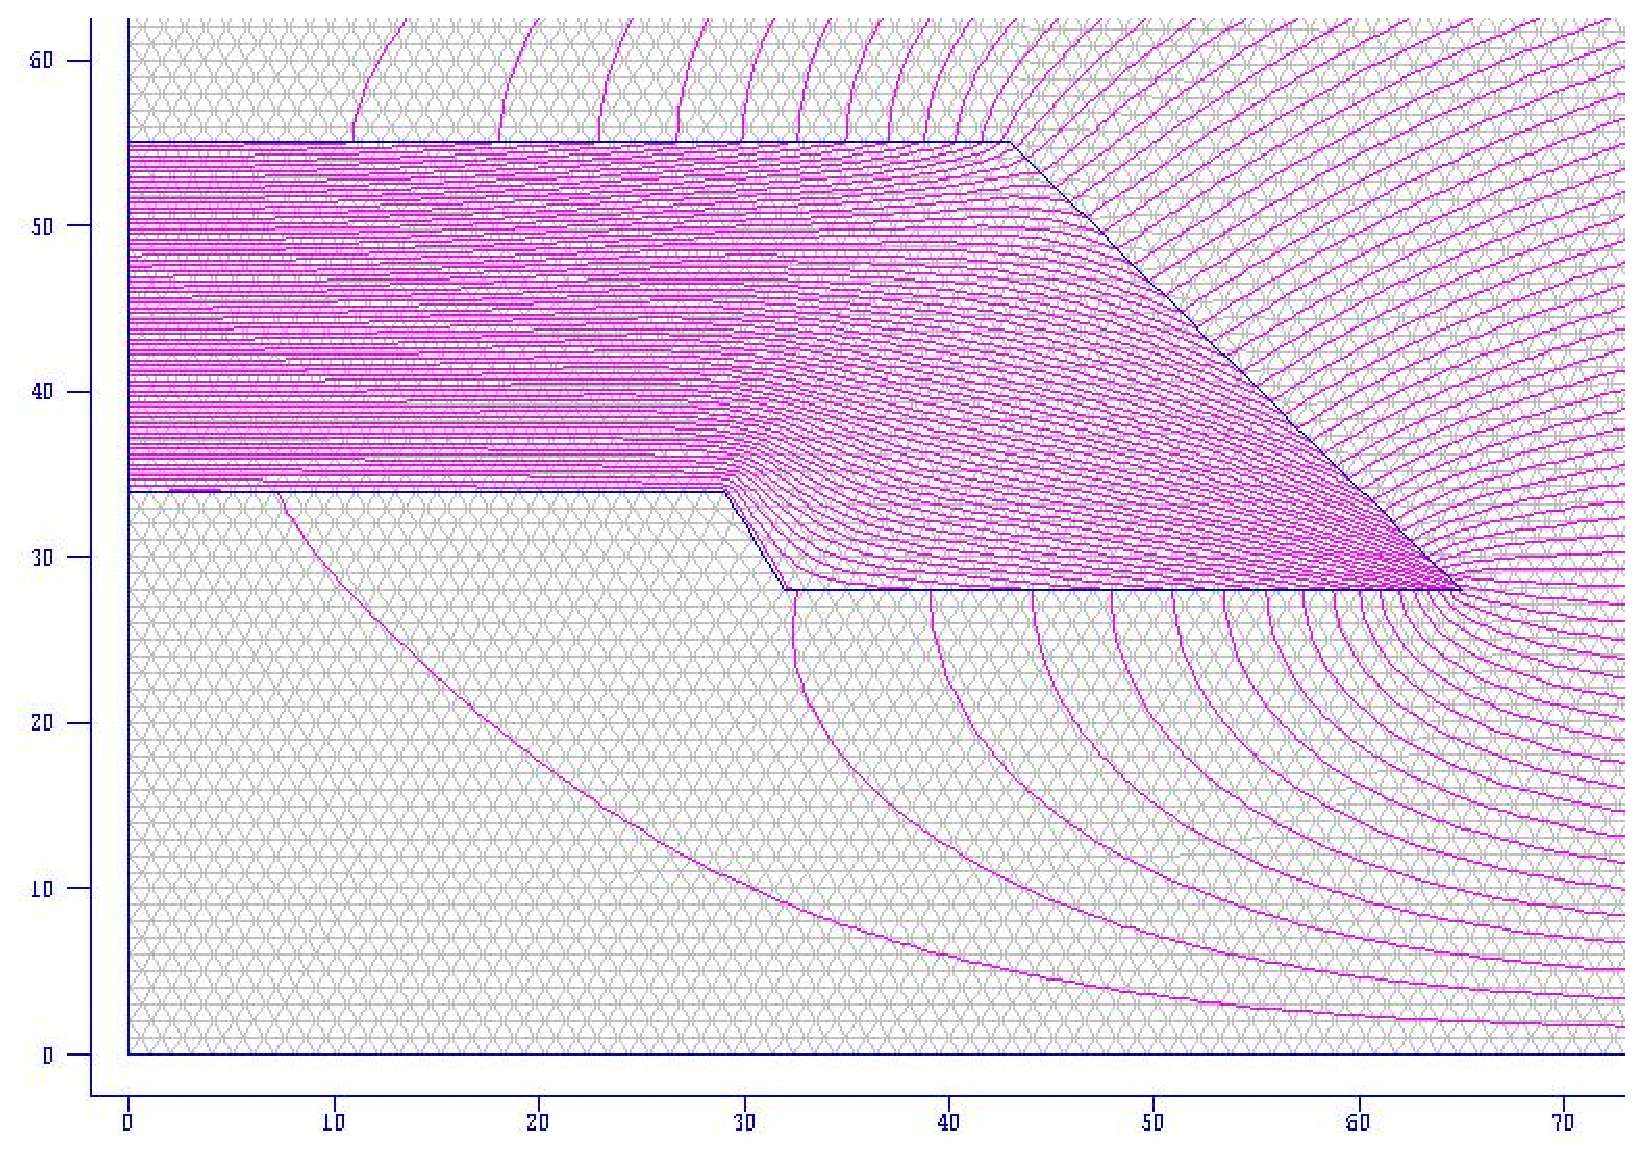
\includegraphics[width=1\textwidth]{Iron_21mm_Shield.eps}
\caption{\small{Magnetic shield  of the 21~mm thick iron  for the downstream
H8500 PMT at an external field of 2500~G}}
\label{Single_Iron_21mm_Shield}
\end{figure}

\newpage
\clearpage

\begin{figure}[ht]
\centering
\subfloat[PMT inner fields]
	{\includegraphics[width=7cm]{H8500_SingleIron_21mm_Thick_PMT_Region.eps}\label{Single_Iron_21mm_PMT_Region}}
\qquad
\subfloat[Iron  inner field]
	{\includegraphics[width=7cm]{H8500_SingleIron_21mm_Thick_Shield_Region.eps}\label{Single_Iron_21mm_Shield_Region}}
\caption{\small{Iron H8500 shield. (a) Magnetic Field within the PMT; (b)
field inside  a 21~mm thick iron shield at varying external magnetic fields. 
This shield is recommended for use in the downstream region of the CTOF counter in 
conjunction with the H8500.}}\label{Upstream_Iron_21mm}
\end{figure}
%

For comparison, the same shield using NETIC instead of iron results in more robust
 behavior shown in Figs.\ref{Single_NETIC_21mm_PMT_Region}
 and \ref{Single_NETIC_21mm_Shield_Region}.
According to these figures  a single NETIC shield of equal thickness 
allows the PMT to operate in a higher magnetic fields up to  2600~G. 



\begin{figure}[ht]
\centering
\subfloat[PMT inner fields]
	{\includegraphics[width=7cm]{H8500_SingleNETIC_21mm_Thick_PMT_Region.eps}\label{Single_NETIC_21mm_PMT_Region}}
\qquad
\subfloat[Netic inner field]
	{\includegraphics[width=7cm]{H8500_SingleNETIC_21mm_Thick_Shield_Region.eps}\label{Single_NETIC_21mm_Shield_Region}}
\caption{\small{Netic shield for H8500.(a) Magnetic field within the PMT;
 (b) Field inside  a 21~mm thick Netic shield at varying external 
magnetic fields. 
}}\label{Upstream_NETIC_21mm}
\end{figure}
%As seen in Fig.~\ref{Single_NETIC_21mm_PMT_Region}, the 
Thus, NETIC shield presents little difference
in performance. In terms of cost, weight, and ease of manufacturing, 
the iron shield is a much more viable selection for the downstream PMT shielding. 
Therefore, an iron shield at a thickness
of 21~mm, an inner radius of 32~mm and an outer radius of 65~mm will be 
considered for use as 
the shield for the downstream H8500 PMT.

\clearpage
\newpage


\susubsection{Proposed PMT Shieldings  in use with the H8500}%%
%
%\paragraph{Proposed Changes to the Upstream PMT Configuration for use with the H8500}
%
If the design is modified to allow 
 the upstream PMTs to be aligned in a staggered configuration, 
it will allow for an additional few~mm of shielding. 
This modification, as well as slightly extending the length of
 the shield, will allow the H8500 to operate well within the
 maximum allowed 200~G external magnetic field. 

The proposed design
 is shown  in Fig.~\ref{Upstream_PMT_Design}. This  shield has
 a thickness of 6~mm, with an inner diameter of 76~mm and an outer 
diameter of 88~mm to the horizontal. This shield  was tested 
in Section-\ref{emsdimen} using both iron and NETIC at a constant
 external magnetic field of 1000~G and varying lengths.

For the downstream PMT, as seen from Fig.~\ref{Single_Iron_21mm_PMT_Region}, 
a single shield of iron with a thickness of 21~mm and an
inner diameter of 68~mm will sufficiently protect the H8500 up to an external
magnetic field of 2500 Gauss. 
%In Fig.~\ref{Single_NETIC_21mm_PMT_Region}, it is shown that
% NETIC will give an additional 5\% in tolerance, allowing the shielded 
%H8500 to operate in an external magnetic field of 2600 Gauss. However,
% this additional shielding is not required, as the downstream H8500 will
% be located in a region where the magnetic field is no greater than
% 2000 Gauss




\newpage
\subsection{Triple Layer Ferromagntic Shield }
%Under current methods of magnetic shielding design for PMTs,
Priliminary consideration with  methods recommended by manufacturers
hints  that   triple shields with thick outer layer may  sufficiently reduce 
the internal magnetic field  in upstream and dowmstream PMTs.
Since the upstream side is  more critical we have started our analythis with the downstream  side. 
Due to restrictions by the  PMT manufacturer, the inner layer is a fixed size and 
material - high permeability mu-metal, similar to  Co-Netic. 
The outermost shield has a maximum of thickness of 1.7~cm due to 
the design constarints. It may be either  soft iron or Netic.


\subsubsection{Downstream Shield for R2983. Pilot design}

The initial design of  the  downstream  shield  is 
shown  in Fig.~\ref{R2083_Initial}.
 This shield  was  tested for its ability to reduce the external 
magnetic field of 1000~G to 
within the tolerance of $0.1G$.
Field map inside the multilayer shield has been  obtained with 
the POISSON-Superfish  program  which performs two-dimensional net calculations 
in a limited space.  A given  axial field inside the cylindrical shield  area   has been
created by a thin solenoid with  significantly larger sizes.
The boundary conditions enforced that the field lines be parallel to
the borders. 
Within these limitations, varying sizes for the middle shield were tested, as well
as the utilizaton of both NETIC and iron in the outer layer.
The corresponding field map at 1000G is  shown  in Fig.~\ref{R2083_Initial}. 
%
% In Fig.\ref{VBT3CYFM} 
%we show a sample of the R2083 shield 
%performance in a 1000G axial field. 
Shown in this figure is a quorter of the full axi-symmetric configuration in the vicinity of the shield   
with the left-down corner being the center of the setup. 
The PMT  occupies the box with coordinate (0,0) and (4.5,2.3)cm  while the  photo cathode is located at  z=4.5cm. 

According to this map, the central  field  of three layer assembly  is  below $0.5$G. 
However,  field  increas towards   open ends of the shield, 
due to a penetrating  axial field lines as seen in Fig.\ref{VBT3CYUS2}.
 At the photo cathode field  reaches  $0.8$G.
We know that  fields  of $0.2-0.5$G are  critical  for  timing PMTs, 
therefore a further optimization has been done in 
Section-\ref{R2083_Triple_No_Coil} in order to achieve fields
 below $\leq0.1$G in the region of the PMT dynode system.



% in hopes that some
%combination would prove effective. 
%The initial shield design is shown in
% Fig.~\ref{R2083_Initial}
%In all of the R2083 models, the models were analized in 
%a cylindrical coordinate system. 


%\subsection{Doubstream Shield perofrmance at  varying  external field}






% In 
%order to determine the saturation of each layer of shielding, the
% collected data points were modified to (0,0), (0,5), (2.3,0), (2.3,5)
% in the PMT region, while the points (2.9,0), (2.9,5) describe the
% inner CONETIC shielding, the points (3.8,0),(3.8,5) describe the
% middle hiperm49 shielding, and the points (5.5,0), (5.5,5) describe
% the outermost shield layer.

\begin{figure}[htbp]
\centering
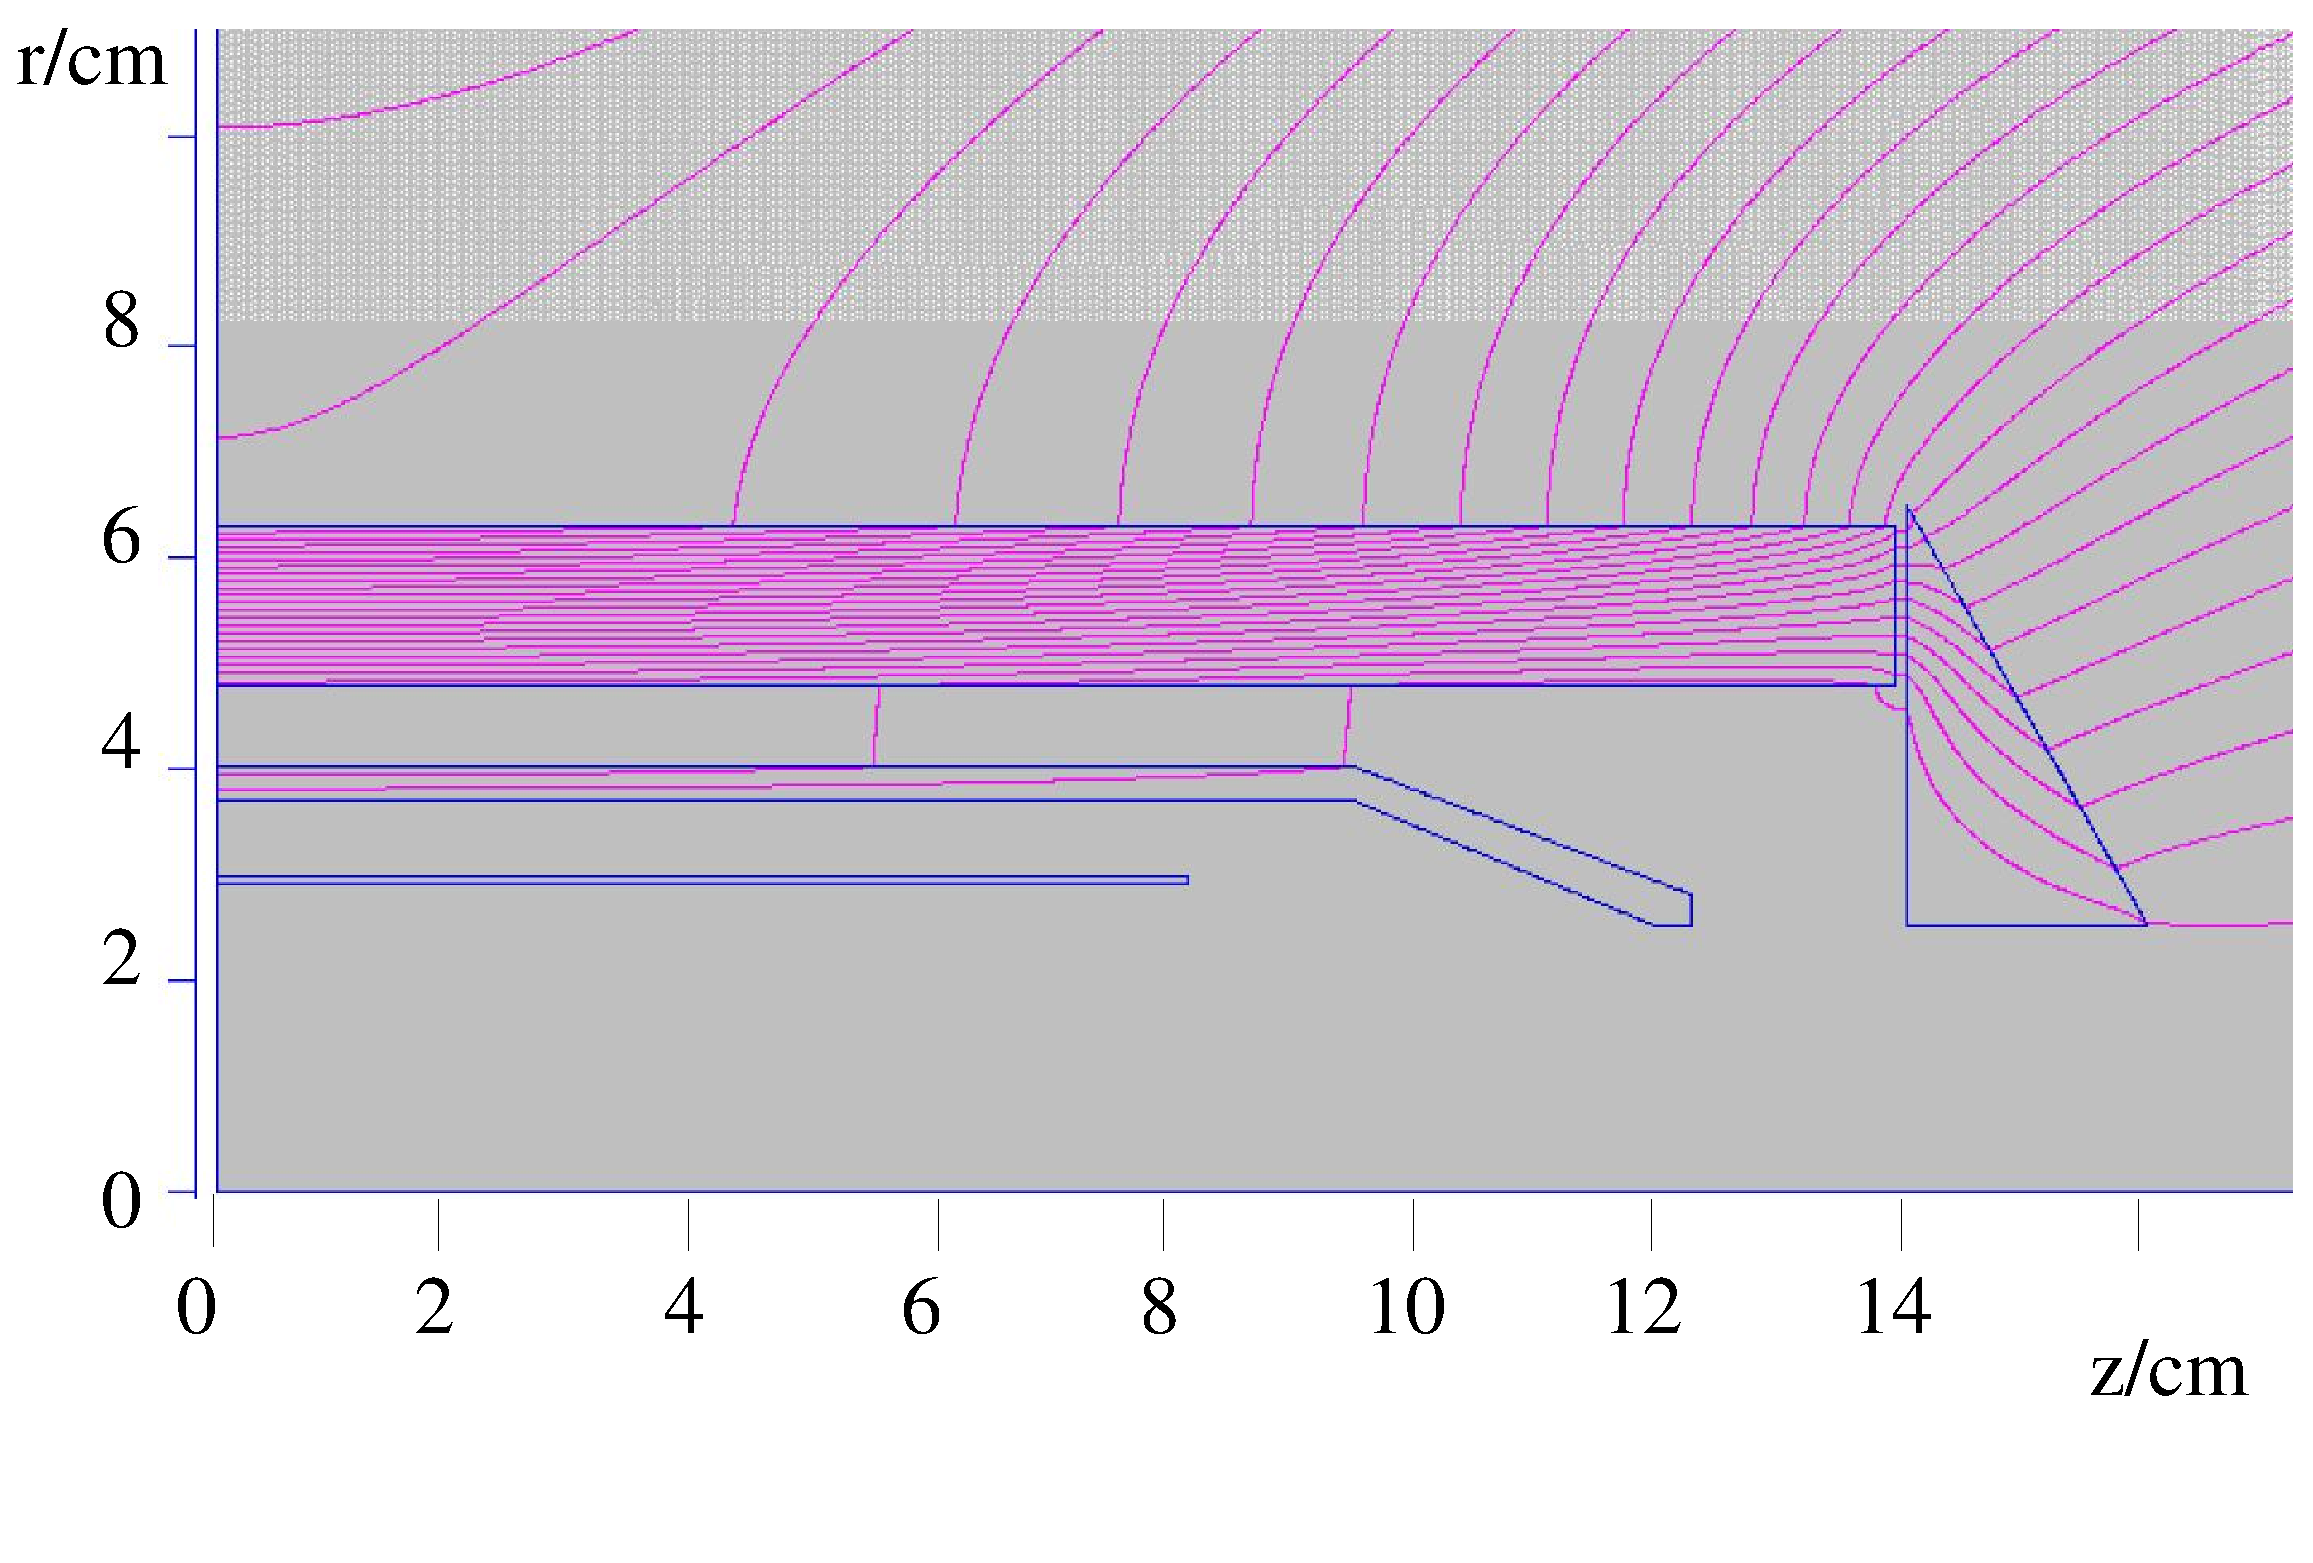
\includegraphics[width=1\textwidth]{R2083_NETIC_hiperm49_CONETIC_standardDesign.eps}
\caption{\small{Initial design of a triple layer magnetic shielding for the R2083.}}
\label{R2083_Initial}
\end{figure}





%\subsection{Example of FEA of  the  ordinary   R2083 shield.}
 %The pilot design of a 3-layer shield for R2083  is shown in Fig.~\ref{VBT3CY}.
%A  high saturation Netic or Soft Iron may  be used for the external layer.
%For the middle layer, the  Hiperm-49 may be used, since it has higher permeability
%at lower fields.  For the inner shielding,  
%a very soft Co-Netic or similar material  will be considered.
%The dimensions and design  will be further optimized via FEA calculations.
%



 
%%%%%%%%%%%%%%%%%%%%%%%%%%%%%%%%%%%%%%%%%%%%%%%%%%%%%%%%%%%%%%%%%%%%%%%%%%%
%\begin{figure}[htbp]
%\centering
%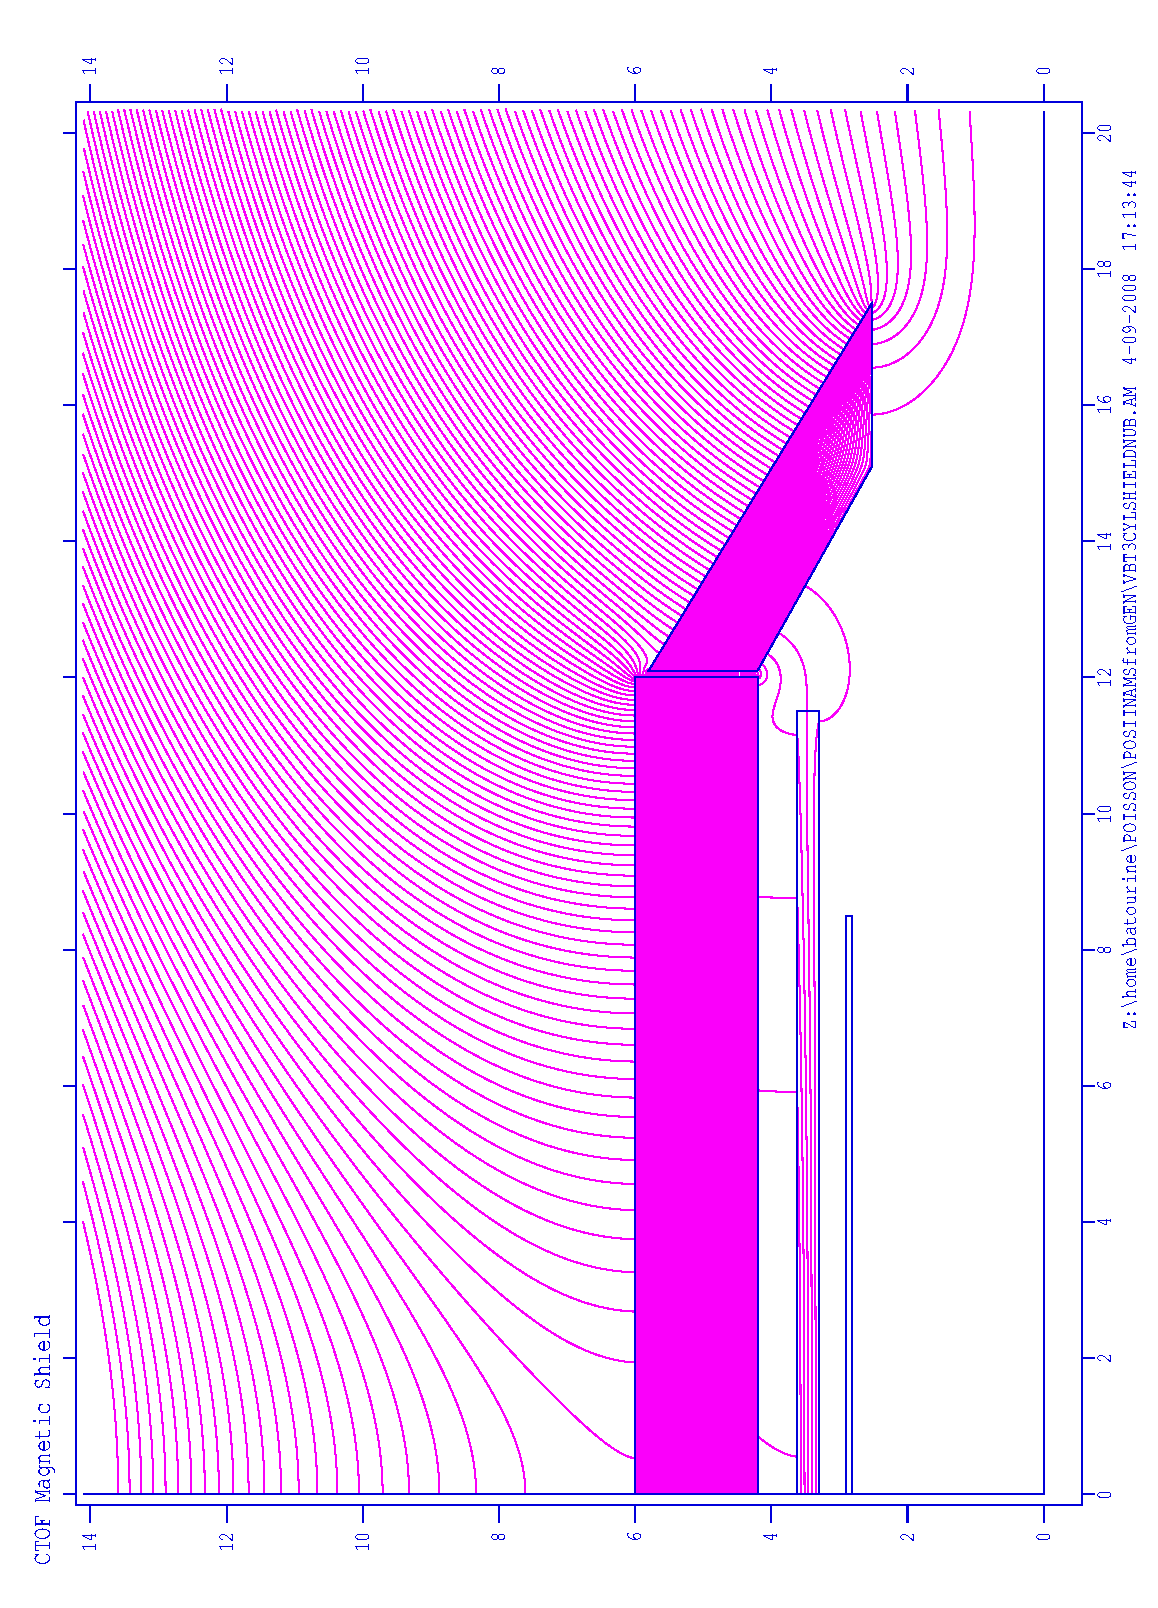
\includegraphics[width=.6\textwidth]{VBT3CYLSHIELDNUB02.eps}
%\caption{\small{
%Sample of a field map for the 3-layer PMT shield 
%in the 1000~G external field.  
%The field in the center is 0.5~G. 
%Axial line is vertical;  radial line is horizontal ; 
%dimensions are given in cm.
%}}
%\label{VBT3CYFM}
%\end{figure}
%%%%%%%%%%%%%%%%%%%%%%%%%%%%%%%%%%%%%%%%%%%%%%%%%%%%%%%%%%%%%%%%%%%%%%%%%%%

%\subsection{R2083 Shield in homogeneous magnetic fields.}

%The pilot  design  for the   R2083 shield is shown in Fig.\ref{VBT3CY}
%As one can see from these calculations the magnetic field inside the
%3 layer shielding does not exceed $0.5G$.
%With this  calculations in hands
%we plan  to purchase  a prototype from the Mu-Shield company, as soon as possible,  and measure the
%internal magnetic field  at various outside fields.
%After that  the second sample will be purchased and the time resolution
% will be determined in the environments of magnetic fields with  one prototyping counter.

%%%%%%%%%%%%%%%%%%%%%%%%%%%%%%%%%%%%%%%%%%%%%%%%%%%%%%%%%%%%%%%%%%%%%%%%%%%%
%\begin{figure}[htbp]
%\centering
%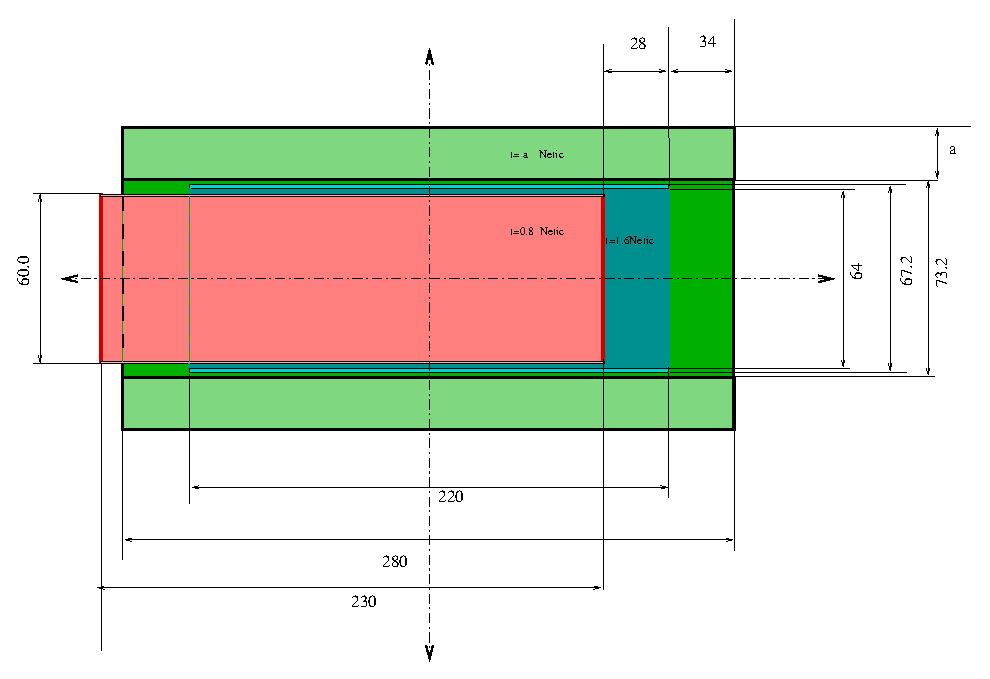
\includegraphics[width=1.0\textwidth]{R2083-3000-ph.eps}
%\caption{The R2083 3 layer  shield design(3R2083l280r732a180).
%The thisckness of the outer cylinder is $a=15mm$, the inner radius is $73.2mm$
%All
%layers are made of Netic ferromagnetic.
%The magnetisation curve for this material is shown in Fig.\ref{muneco}.}
%\label{barrel}
%\end{figure}
%\clearpage
%\newpage
%%%%%%%%%%%%%%%%%%%%%%%%%%%%%%%%%%%%%%%%%%%%%%%%%%%%%%%%%%%%%%%%%%%%%%%%%%%




\subsubsection{Downstream Shield for R2083 in varying field} 
\label{R2083_Triple_No_Coil}
In the initial shield design in Fig.~\ref{R2083_Initial}, the middle shielding 
layer is composed of 0.3~cm of hiperm49, while the outermost layer is composed
 of 1.5~cm thick of either iron or NETIC. Both outer shield materials were
 tested at varying magnetic fields, from 250~G to 1250~G, in increments of 250~G.

In our tests we  monitor the following  points inside PMT:
   (0,0) and (2.3,0) at  the median plane with the  first PMT dynode;
   (0,5) and (2.3,5) at  the PMT entry window.
In order to avoid  saturation effects we monitir the bulk of ferromagnetics:
 (2.9,0) and (2.9,5) - inner layer; 
 (3.8,0) and (3.8,5) - middle layer; 
(5.5,0) and (5.5,5)  - outer layer.
All points are given in (r,z) form and are expressed in centimeters.





The  magnetic field of 700~G  was depressed up to 0.4-0.9~G in the shielded
 region of iron shield, as seen in Fig.~\ref{R2083_Initial_Iron_PMT_Region}. 
Inside the Netic 
 shield   residual field ranges from 0.4~G to 0.9~G at higher field 0f 850G,
 as seen  in Fig.~\ref{R2083_Initial_NETIC_PMT_Region}.

These values are  significantly  higher of  required values  even 
at  twice lower external fields . Morevover,
the outer shield layer is already at its maximum 
thickness as allowed by the current CTOF design. 

The only possibility for improvement is by increasing the thickness 
of the middle layer of hiperm49 from 0.3~cm to the maximum allowed by the design 
of 0.8~cm. In Fig.~\ref{R2083_Triple_0.8cm_PMT_Region}, it is shown 
that even with an outer layer of NETIC at 1.5~cm thick and a middle layer 
of hiperm49 at 0.8~cm thick, the maximum allowed by the current CTOF design, 
it is not possible to decrease the internal magnetic field to below 0.1~G. 


\begin{figure}[ht]
\centering
\subfloat[PMT inner field]
	{\includegraphics[width=7cm]{R2083_Iron_hiperm49_CONETIC_0.3mm_PMT_Region.eps}\label{R2083_Initial_Iron_PMT_Region}}
\qquad
\subfloat[Ferromagnetic magnetisation in the external layer.]
{\includegraphics[width=7cm]{R2083_Iron_hiperm49_CONETIC_0.3mm_Outer_Region.eps}\label{R2083_Initial_Iron_Outer_Region}}
\qquad
\subfloat [Magnetisation of the middle  layer.]
{\includegraphics[width=7cm]{R2083_Iron_hiperm49_CONETIC_0.3mm_Middle_Region.eps}\label{R2083_Initial_Iron_Middle_Region}}
\qquad
\subfloat[Magnetisation of the inner  layer.]
{\includegraphics[width=7cm]{R2083_Iron_hiperm49_CONETIC_0.3mm_Inner_Region.eps}\label{R2083_Initial_Iron_Inner_Region}}
\caption{\small{Magnetic fields in the PMT and shield regions using a triple layer Iron-hiperm49-CONETIC shield at varying external magnetic fields for the R2083. The middle layer of hiperm49 is 0.3~mm thick.}}\label{R2083_Initial_Iron}
\end{figure}
\clearpage
\newpage

%% Figures for NETIC R2083 initial start here

\begin{figure}[ht]
\centering
\subfloat[PMT Region]
	{\includegraphics[width=7cm]{R2083_NETIC_hiperm49_CONETIC_0.3mm_PMT_Region.eps}\label{R2083_Initial_NETIC_PMT_Region}}
\qquad
\subfloat[ Magnetisation of the external layer]
{\includegraphics[width=7cm]{R2083_NETIC_hiperm49_CONETIC_0.3mm_Outer_Region.eps}\label{R2083_Initial_NETIC_Outer_Region}}
\qquad
\subfloat[Middle layer magnetisation.]
{\includegraphics[width=7cm]{R2083_NETIC_hiperm49_CONETIC_0.3mm_Middle_Region.eps}\label{R2083_Initial_NETIC_Middle_Region}}
\qquad
\subfloat[Inner layer magnetisation.]
	{\includegraphics[width=7cm]{R2083_NETIC_hiperm49_CONETIC_0.3mm_Inner_Region.eps}\label{R2083_Initial_NETIC_Inner_Region}}
\caption{\small{Magnetic fields in the R2083 PMT and shield regions using 
a triple layer NETIC-hiperm49(3mm)-CONETIC shield at 
varying external magnetic fields.}}
\label{R2083_Initial_NETIC}
\end{figure}
\clearpage
%\newpage

\begin{figure}[ht]
\centering
\subfloat[PMT Region]
	{\includegraphics[width=7cm]{R2083_NETIC_hiperm49_CONETIC_0.8mm_PMT_Region.eps}\label{R2083_Triple_0.8cm_PMT_Region}}
\qquad
\subfloat[Outer Shield Region]
{\includegraphics[width=7cm]{R2083_NETIC_hiperm49_CONETIC_0.8mm_Outer_Shielding_Region.eps}\label{R2083_Triple_0.8cm_Outer}}
\qquad
\subfloat[Middle Shield Region]
{\includegraphics[width=7cm]{R2083_NETIC_hiperm49_CONETIC_0.8mm_Middle_Shielding_Region.eps}\label{R2083_Triple_0.8cm_Middle}}
\qquad
\subfloat[Inner Shield Region]
{\includegraphics[width=7cm]{R2083_NETIC_hiperm49_CONETIC_0.8mm_Inner_Shielding_Region.eps}\label{R2083_Triple_0.8cm_Inner}}
\caption{\small{Magnetic fields in the PMT and shield regions using a 
triple layer NETIC-hiperm49(8mm)-CONETIC shield at varying external magnetic fields. 
}}
\label{R2083_Initial_Thick_NETIC}
\end{figure}
\clearpage
\newpage

From these considerations we conclude that  a  triple shielding  is  not  
sufficient for the R2083 in the invironments of the CTOF detector,
even at lower fields 
%Due to the design constarins 
It looks like  the last resort of ferromagnetic shields  is exhausted.

However,  we have succeded to  develope hybrif ferromagnetic  shield using 
a new  approache described in the following Section-\ref{novelle}
Such shield allows  to attain fields below 0.1G in both  upstream and
downstream PMTs.




\newpage

\section{Novelle Dynamical Magnetic Shields with Compensating Coil.}

\label{novelle}
As it was shown in the previous section the PMT inner field 
strongly depends on the ferromagnetic permeability, which is  sensible to
 fabrication technologies and applied magnetic fields, as well.


\subsection{Basic idea and design}

Our main idea is to control the magnetisation of shield cylinder
using active elements such as coils or solenoids wind  around the 
ferromagnetic components.
%With the purpose of attaining fields below 0.1G we suggest to use a
We call the  combination  of passive  and active elements of shielding as hybrid
shield or dynamical shield.  With the purpose of attaining fields below 0.1G
we have studied the performance of  hybrid   shield with the POISSON program.


On Fig.\ref{VBT3CYUS1} we present the  design and the fieldmap  
for the Hybrid magnetic shield
with a compensating coil inside the shield assembly. 
The coil is placed between the  the middle and the inner layers.
The detailed magnetic field map of this shield  is shown in Fig.\ref{VBT3CYUS2}.

\subsection{Upstream dynamical shield}
As seen from this figure the  field inside the PMT region is  far  below 0.1G,  
while the  external field is as high as 400G. Therfore this  shield may be used at the 
upstream side of the CTOF detector.
%
%According to the model  shown in Fig.\ref{VBT3CYUS1}
%a relatively small  current
%below  1A  in   ~1mm thick wire is enough
%to reduce the inner PMT  field  below 0.1G.
%This conclusion is of high  practical importance since the
%DC is limited by $~/approx2A$ per mm^2.
%
%In the  model shown in Fig.\ref{VBT3CYUS1}
The total current  throught the compensating  coil is  $\approx100A$,
while  the coil is  $\approx200mm$ long.
Thus, the coil  may consit of  200 winds  of 1mm thick wire  with a current of .5A, only, which means a very low power dissipation.
This conclusion is of high  practical importance since, in order to avoid overheating,
 the  DC has to be  limited by $~\approx 2A$ per mm$^2$.
Certainly,  higher fields may be  exterminated with a higher
currents in the  compensation coil.

Thus, Hybrid Magnetic Shields are very promising, therefore
we have  further  developed   and poprototyped  such shields.
Below we describe our first practical tests with hybrid magnetic shield prototypes.

\subsection{Prototyping and Testing.}

In this section  we describe two  prototypes for  the inner layer of the hybrid
 magnetic shield.  Prototype are the ferromagnetic cylinders
instrumented  with the external  compensating coils.
Ferromagnetic proprties of prototypes are  different.
Their  performance was studied  at    magnetic fields below 100G using Helmholz coils.
Such fields are  expected  after  two  external layers of  a tryple  shield.
%The almost uniform external field was produced by the Helmhols Coils 2m in diameter. 
The Gaussmeter was placed in the center of the
shiled. On our tests we observed the inner field with the
Gaussmeter varying the current in the compensationg coil at given external field.

\paragraph{Measurements with Hyperm-49 prototype}
First   prototype is the Hiperm-49 200~mm long tube,  
1.6~mm thick with the inner radius 75mm.
The compensationg coil consists of 108
 turns of $~1$mm thick wire wind around the ferromagnetic tube.
 The internal field of this  prototype vs the coil current 
 was tested at external field
75~G  produced by Helmholz coils. 
The result is shown  in Fig.\ref{hypermdysh}.
As one can see from this figure, the inner field 
drops to zero with encreasing current, then it
encrease  with  significantly lower rate.

\paragraph{Measurements with $\mu$-metal prototype}
The second prototype is the $\mu$-metal cylinder  150~mm in inner  diamter 0.8~mm  thick.
The external compensating coil consists of 50 winds of 2mm thick wire.
The inner field in function on the coil current  at 35G  external field  is
shown  in Fig.\ref{mumedysh}. Zero inner field has been achieved  at   
$\approx$0.9A, then it climbs with the same rate.  
Hence, due to a higher permeability and, perhaps,
significanltly  lower  Hysteresis effects, 
the $\mu$-metal exhibits   more regular behavior than  Hyperm-49.

Thus, our first practical tests shows the vitality of
the idea of using compenstion coils. The practical realisation of such 
shielding looks easy, since in order to exterminarte fields of 50-100G
only one layer of winding is required, while the curren troughthe vireis
quite  low.
%\newpage
%\end{document}
%\subsubsection{POISSON tests.}
%This section is reserved for the POISSON  analythis of the performance of the 
%Hybrid Shield prototype   varying the external fieled.
%Inner field in function on the coil current is shown in Fig.\ref{dynashpois1}.
%At given value  of the external field  the  field inside the magnetic shield was minimized 
%at certain current.  Thus determoned  current in   function on the external field
% is  shown  in Fig.\ref{dynash}.
%%%%%%%%%%%%%%%%%%%%%%%%%%%%%%%%%%%%%%%%%%%%%%%%%%%%%%%%%%%%%%%%%%%%%%%%%%%%
\begin{figure}
\centering
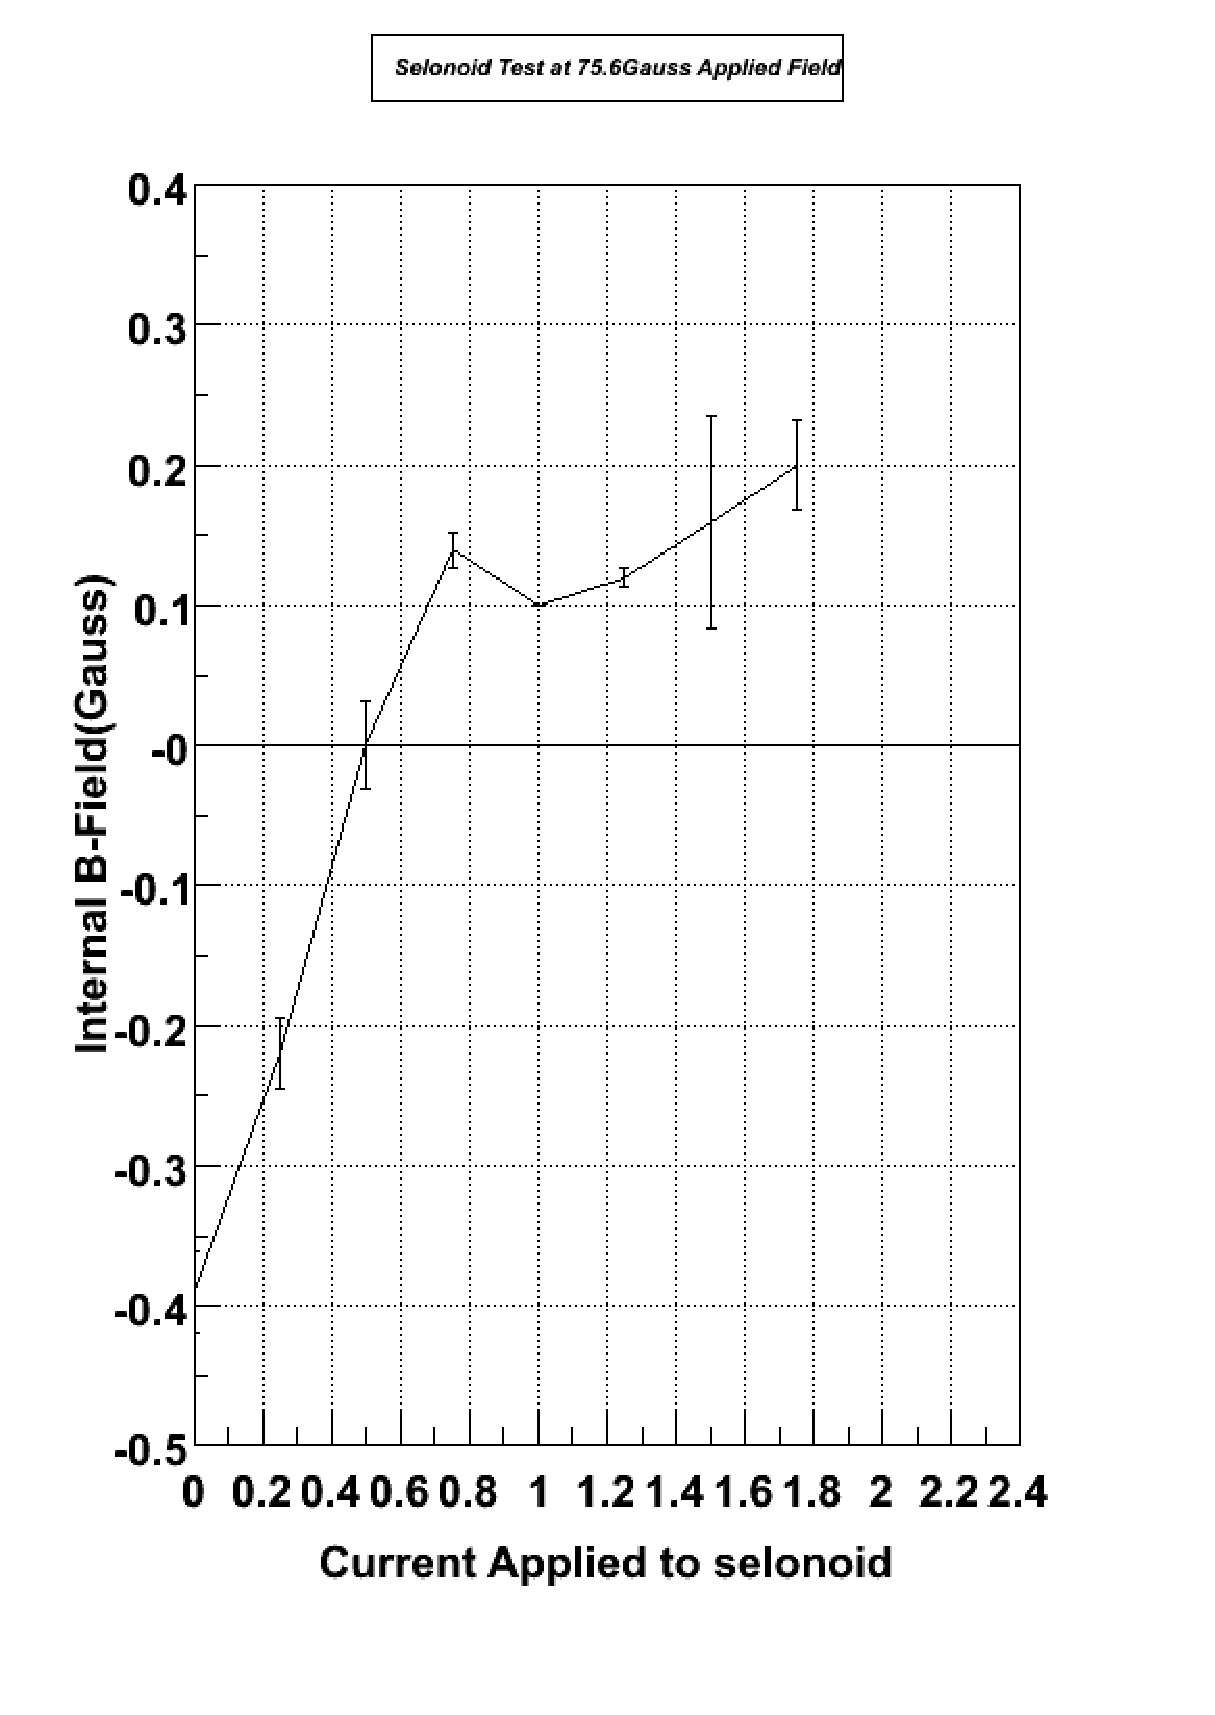
\includegraphics[width=.6\textwidth]{75.6_gauss.eps}
%\includegraphics[width=.6\textwidth]{HyMagSh400G.eps}
\caption{\small{ Performance of the inner layer of  Magnetic Shield for R2083
with the compensating coil. Zero inner field has been  achieved at $I\approx0.5$A }}
\label{hypermdysh}
\end{figure}
%%%%%%%%%%%%%%%%%%%%%%%%%%%%%%%%%%%%%%%%%%%%%%%%%%%%%%%%%%%%%%%%%%%%%%%%%%%
\begin{figure}
\centering
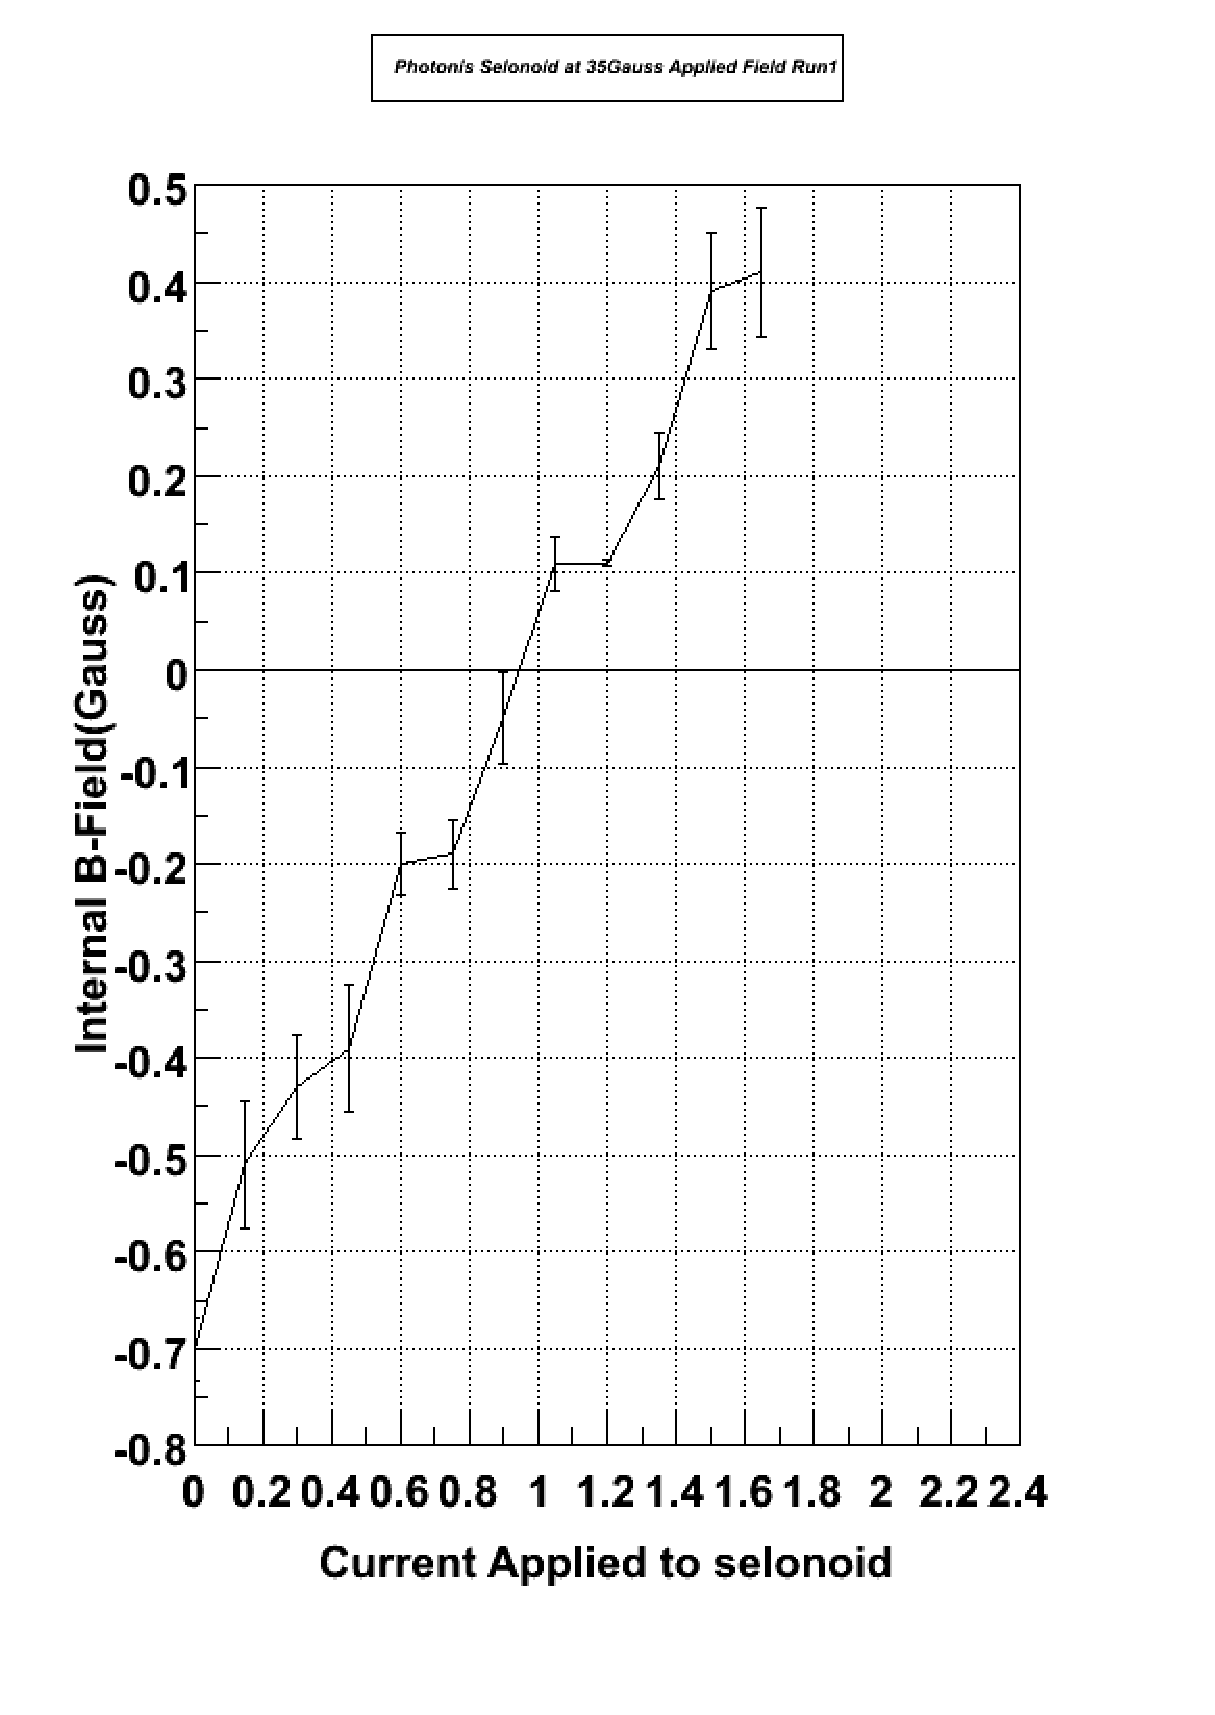
\includegraphics[width=.6\textwidth]{35_gauss_run1.eps}
\caption{\small{Inner $\mu$-metal layer of  magnetic shield 
with the compensating coil. Zero  field has been  achieved at $I\approx0.9$A}}
\label{mumedysh}
\end{figure}
%%%%%%%%%%%%%%%%%%%%%%%%%%%%%%%%%%%%%%%%%%%%%%%%%%%%%%%%%%%%%%%%%%%%%%%%%%%
\begin{figure}[htbp]
\centering
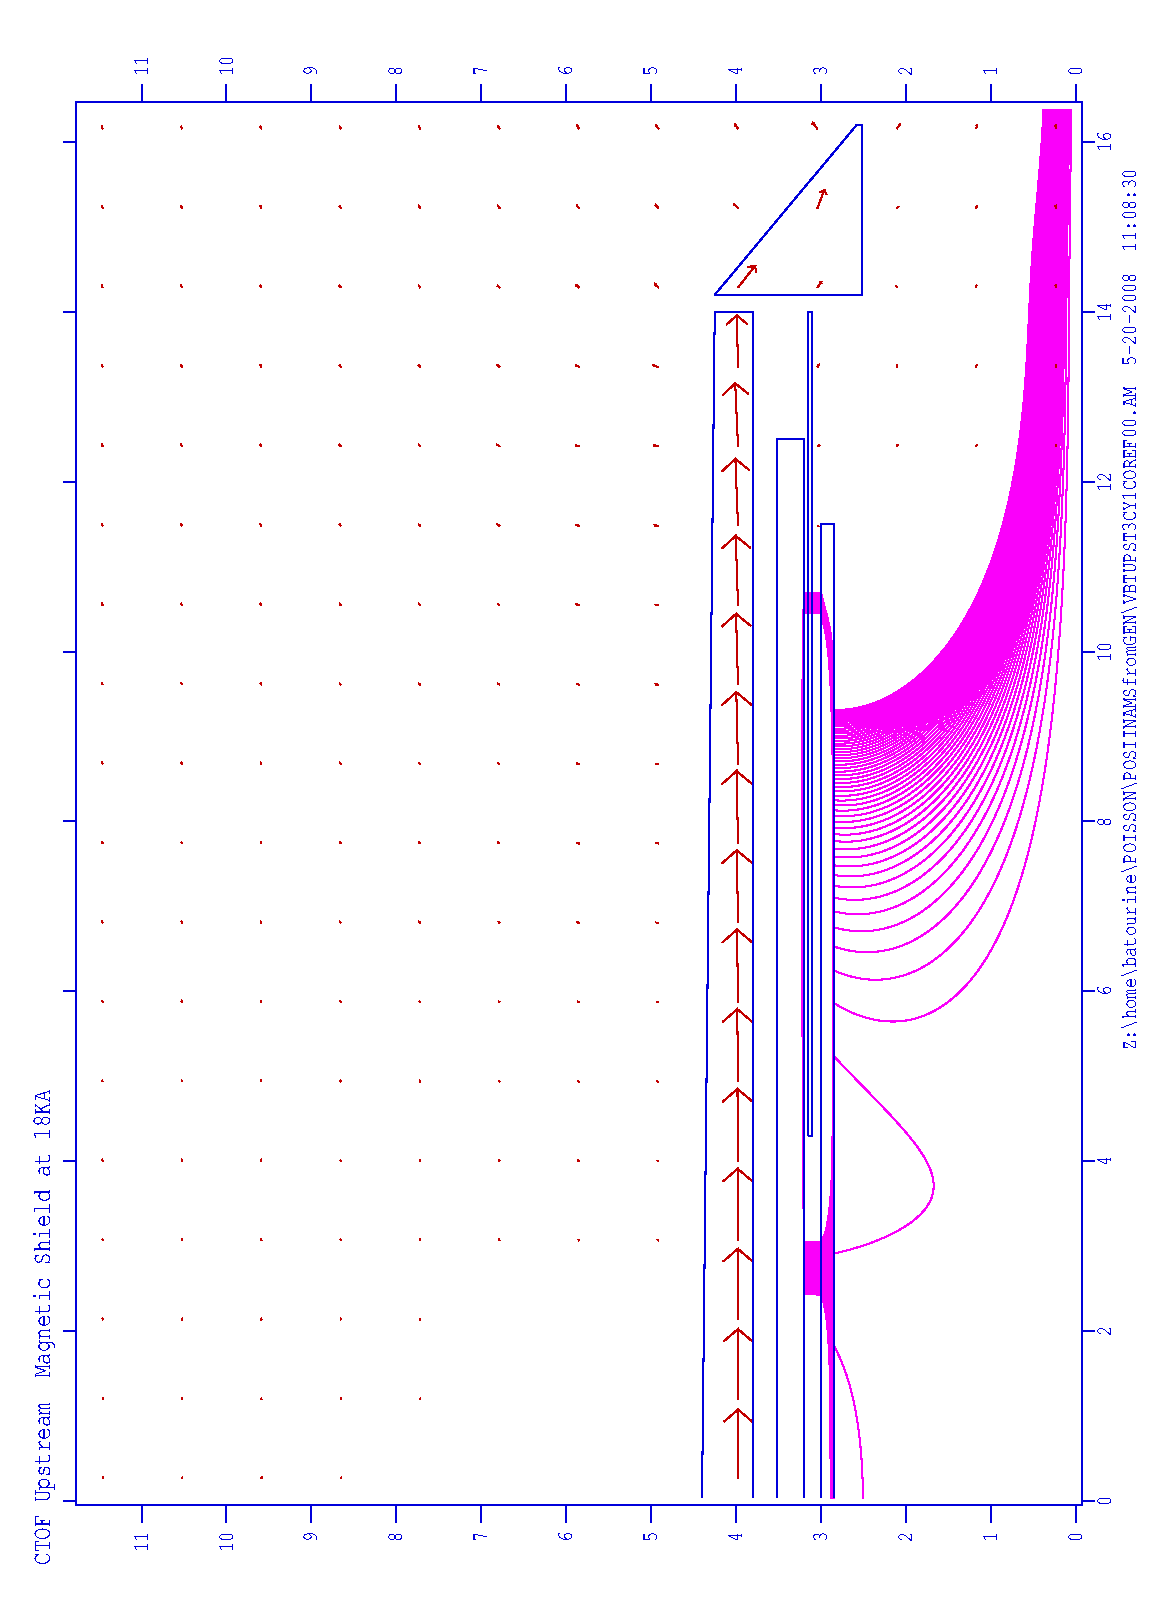
\includegraphics[width=.6\textwidth]{VBTUPST3CY1COREF0001.eps}
%\includegraphics[width=.6\textwidth]{HyMagSh400G.eps}
\caption{\small{ Field map inside the Hybrid Magnetic Shield for R2083
with the compensating coil. The coil has ~100 winds around  the H2431 assembly.
At   the 400~G external field the inner PMT field  is far  below $0.1$G.}}
\label{VBT3CYUS1}
\end{figure}
%%%%%%%%%%%%%%%%%%%%%%%%%%%%%%%%%%%%%%%%%%%%%%%%%%%%%%%%%%%%%%%%%%%%%%%%%%%
%%%%%%%%%%%%%%%%%%%%%%%%%%%%%%%%%%%%%%%%%%%%%%%%%%%%%%%%%%%%%%%%%%%%%%%%%%%
\begin{figure}[htbp]
\centering
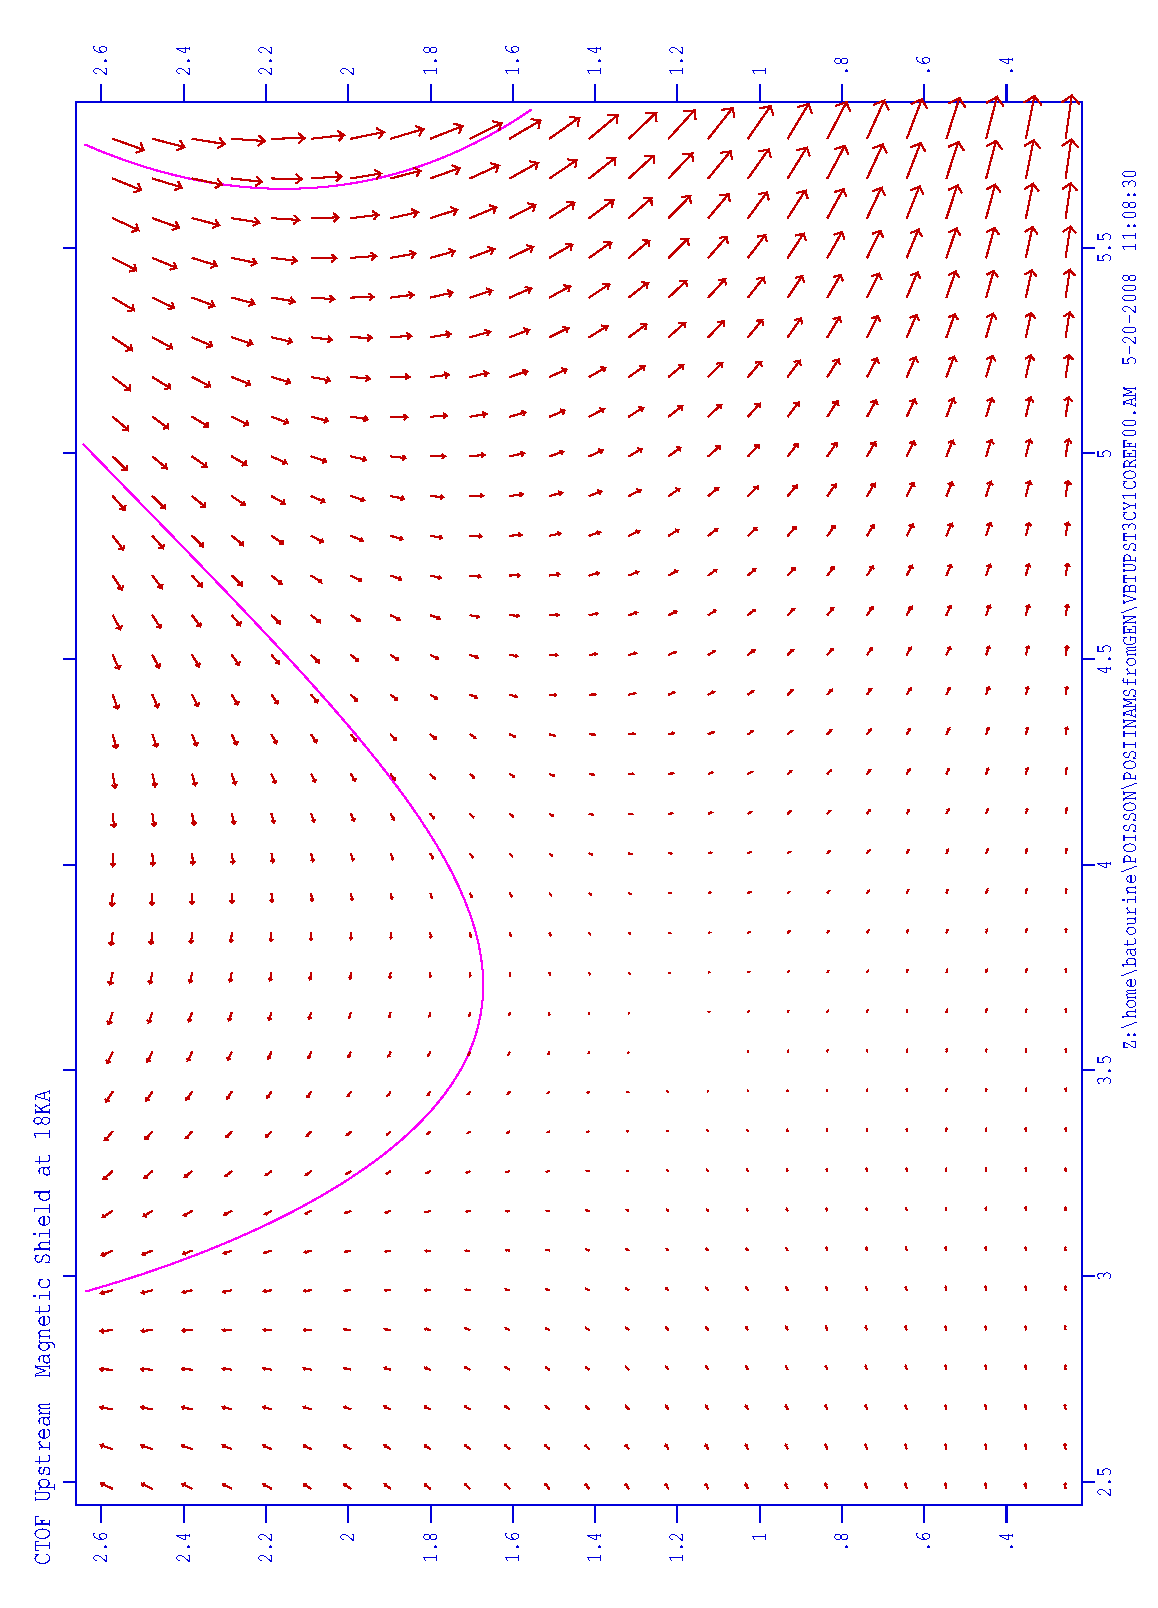
\includegraphics[width=.6\textwidth]{VBTUPST3CY1COREF0002.eps}
\caption{\small{  ``Zoommed in'' field map inside the R2083 Hybrid Magnetic Shield.
with the compensating solenoid around H2431 assembly. External field is 400G.
The length of arrows indicate the magnitude of magnetic field. 
The maximum field corresponding to the longest arrow  is $\approx$1G.
In the region of the  PMT photocathode ($z=4cm$)  the inner PMT field
is far  below  0.1G.}}
\label{VBT3CYUS2}
\end{figure}
%%%%%%%%%%%%%%%%%%%%%%%%%%%%%%%%%%%%%%%%%%%%%%%%%%%%%%%%%%%%%%%%%%%%%%%%%%%




\subsection{Downstream Tapered  Shield}

In our previous calculations, it was observed that the 
internal B-field  in the outermost shielding layer was 
non-uniform across the length of the shield, becoming greater
towards the median of the cylinder.
This effect may be seen at any calculated field map as follows.
We observe that
field lines are captured  by the outer cylinder almots perpendicular
to its surface. Then all lines
run  almost parallel to the axis. Therefore  magnetic flux density 
increase, rougly linearly, 
towards the median of the cylinder. Thus, the  most dangerous place,
where the  effect of  ferromagnetic saturation 
shows up first, is just  the meadian plane, where the field lines penetrate
through a ``hole'' created by a saturated ferromagnetic. This effect also
explains the effect of shield collaps at high shield length. 

 In order to reduce  this  effect we suggest an improved shield 
 that involves the use of a tapered outer cylinder the   thickness of which  
linearly increase  towards the median plane.
% in combination with the 
%correction coil between the inner and middle layers of CONETIC and Hiperm-49 shielding was tested. 
This new  design with  correction coil   is shown in
 Fig.~\ref{Tapered_Shield_Design}.
% Due to its availability by the manufacturer, NETIC cannot be used 
%as a material for the outermost shield, as it is available only in sheets. 
%Therefore, 
The outermost  shield is composed of iron, beginning with a thickness of 1.0~cm and slowly thickening 
to 1.7~cm thick.  The middle layer is made of Hiperm-49(3mm)  while  the inner layer is CONETIC(0.8mm)
and the external magnetic field is kept constant at 1000~G.

%Initially, this design was tested with a middle layer of 0.5~cm thick of hiperm49.
% Figure \ref{Tapered_Shield_0.5cm_PMT_Region} depicts the internal magnetic field, 
%while Figs.~\ref{Tapered_Shield_0.5cm_Outer_Region},~\ref{Tapered_Shield_0.5cm_Middle_Region},
% and~\ref{Tapered_Shield_0.5cm_Inner_Region} shows the saturation inside the three layers of
% shielding. The POISSON models show that it is possible to bring the entire PMT region to below
% 0.1~G when the correction coil curent is set at $\approx 27$~A. It is interesting to observe
% that as the current increases, the saturation inside the innermost CONETIC layer decreases,
% which is counter to previous studies.


%Following the successful testing of this design, the thickness of the middle layer was reduced
% from 0.5 cm thick to 0.3 cm thick  for the purpose of weight and cost. 

In Fig.~\ref{Tapered_Shield_0.3cm_PMT_Region},
it is observed that the internal magnetic field of the PMT region is below 0.1 G when the correction coil current 
is set between $25-30$A. It is also of interest to note that at this high magnetic field, none of the shields have
 reached saturation, as depicted in Fig.~\ref{Tapered_Shield_0.3cm_Outer_Region}, Fig.~\ref{Tapered_Shield_0.3cm_Middle_Region},
 and Fig.~\ref{Tapered_Shield_0.3cm_Inner_Region}.




%\begin{figure}[htbp]
%\centering
%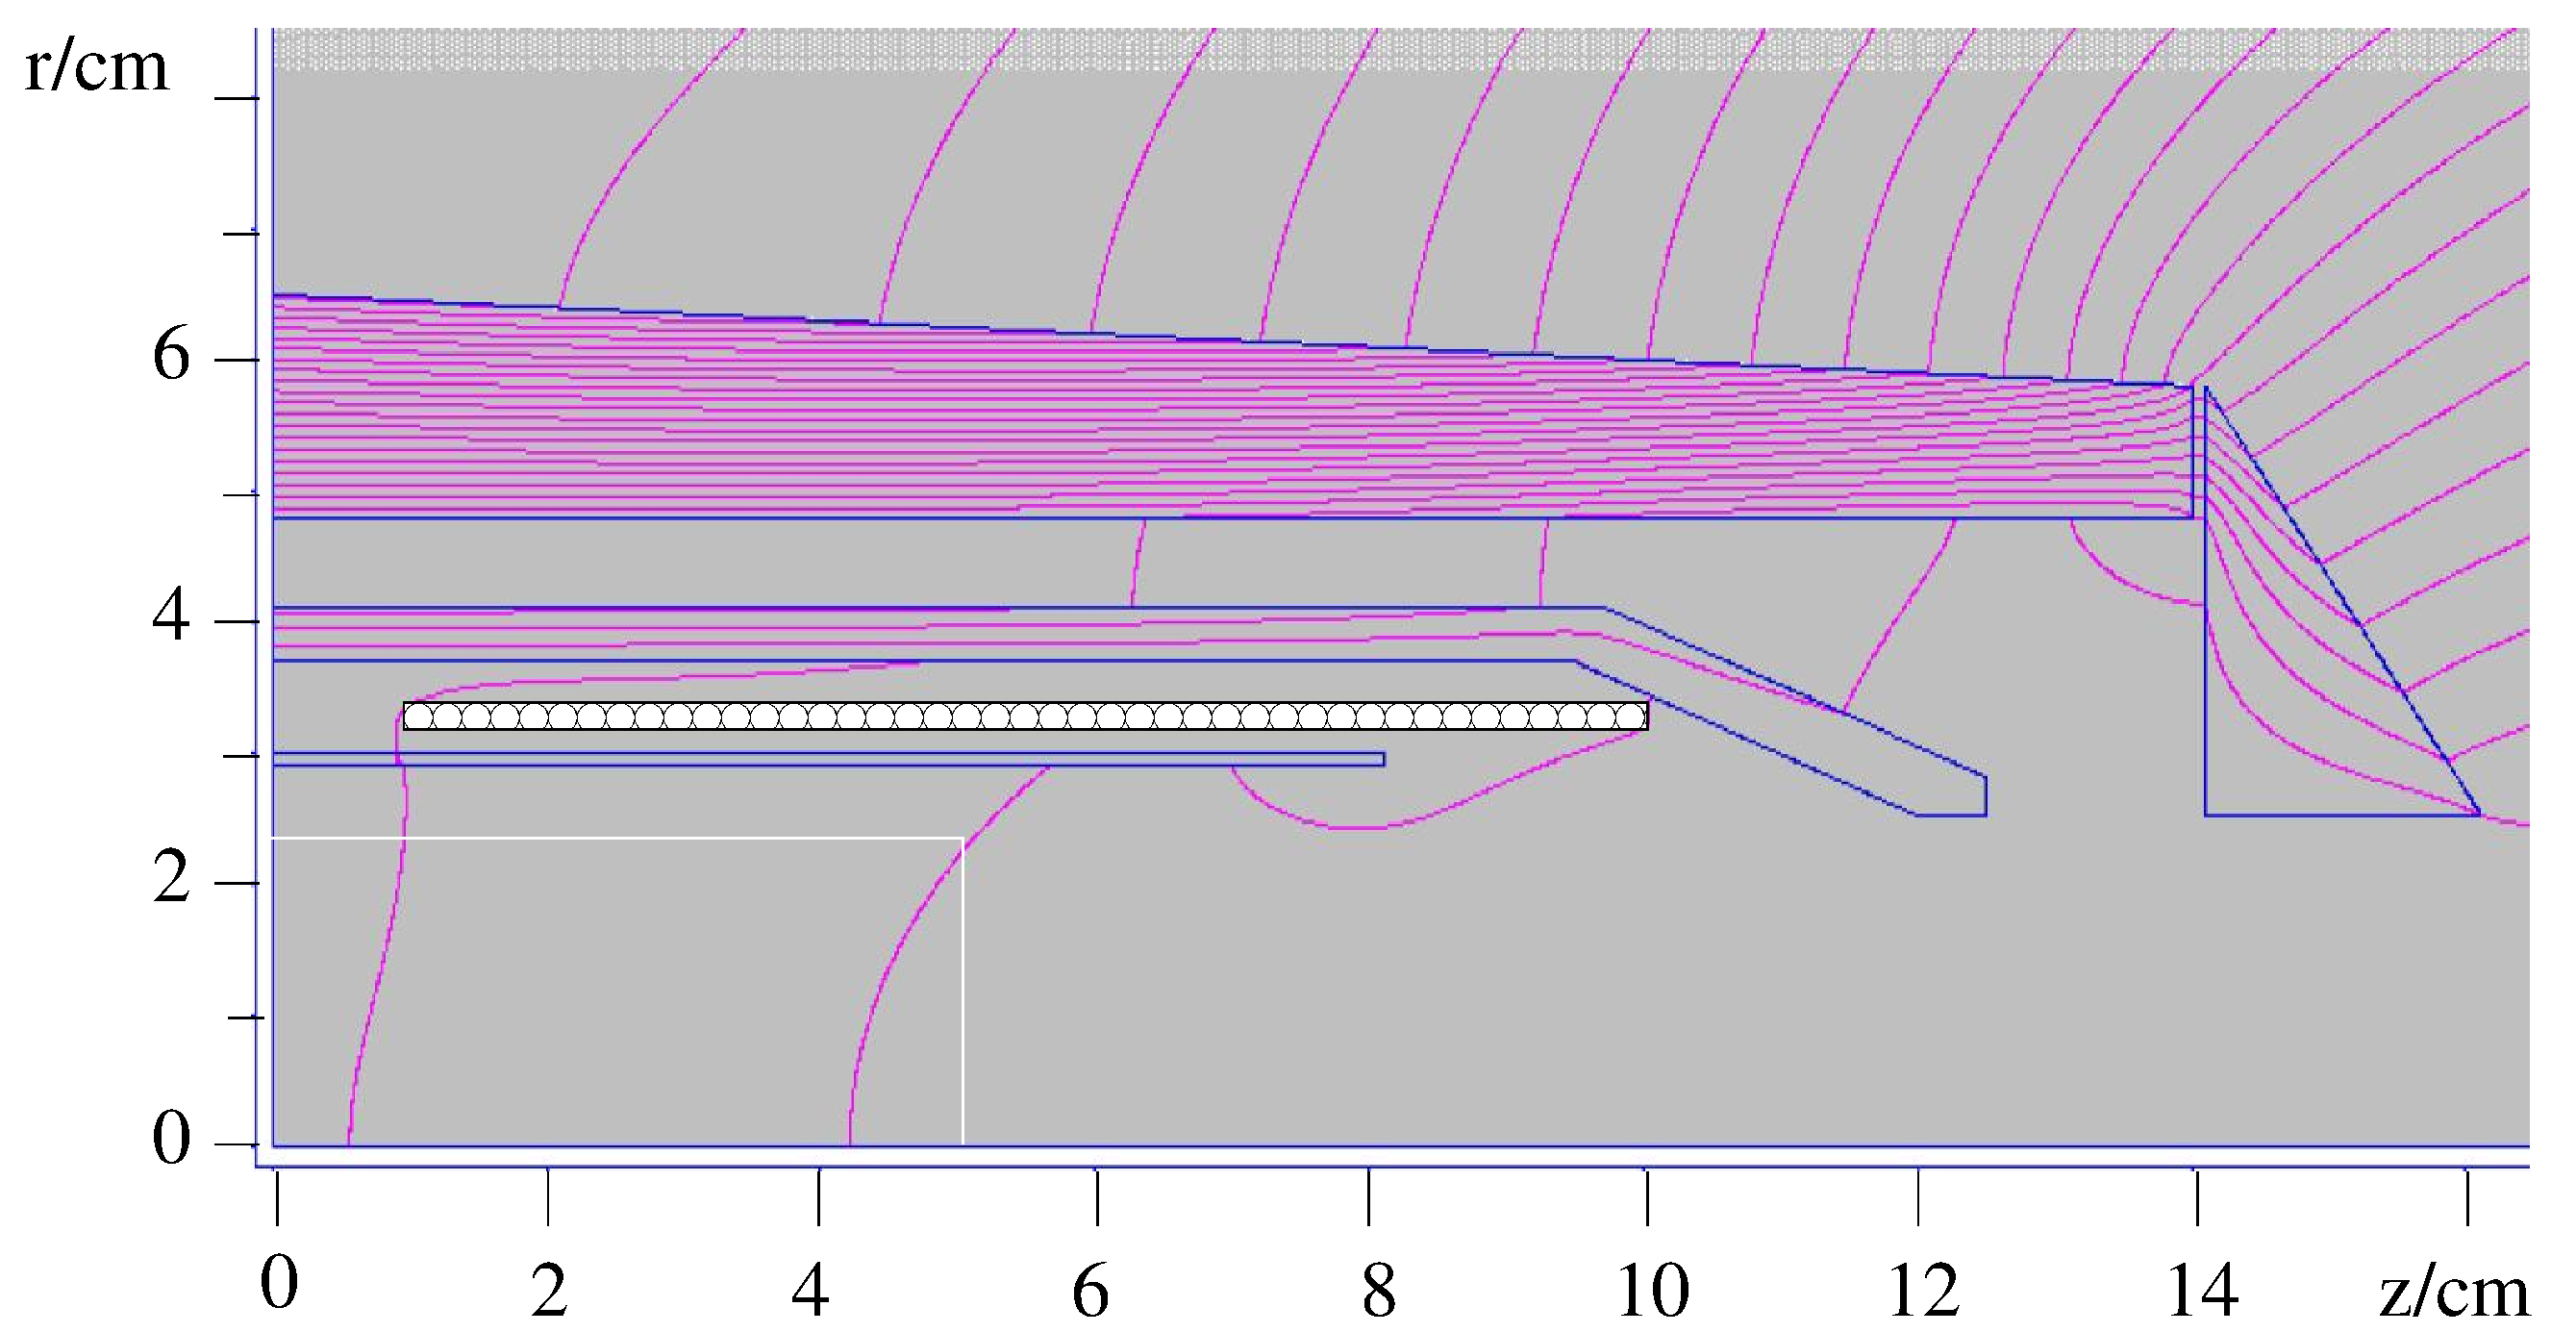
\includegraphics[width=0.7\textwidth]{R2083_Iron_hiperm49_CONETIC_TaperedShieldDesign.eps}
%\caption{\small{Initial design of tapered shield with correction coil. The outermost shield is made of iron while the middle shield is made of hiperm49. The external magnetic field is set at 1000 G and the graph here is shown when the correction coil is set to 25 A.}}
%\label{Tapered_Shield_Design}
%\end{figure}
%% Figures for 0.5cm thick hiperm49 shield*

%\begin{figure}[ht]
%\centering
%\subfloat[PMT Region]
	%{\includegraphics[width=7cm]{R2083_Tapered_0.5cmMiddle_PMT_Region.eps}\label{Tapered_Shield_0.5cm_PMT_Region}}
%\qquad
% \subfloat[Outer Shield Region]
	%{\includegraphics[width=7cm]{R2083_Tapered_0.5cmMiddle_Outer_Shielding_Region.eps}\label{Tapered_Shield_0.5cm_Outer_Region}}
%\qquad
%\subfloat[Middle Shield Region]
	%{\includegraphics[width=7cm]{R2083_Tapered_0.5cmMiddle_Middle_Shielding_Region.eps}\label{Tapered_Shield_0.5cm_Middle_Region}}
%\qquad
%\subfloat[Inner Shield Region]
	%{\includegraphics[width=7cm]{R2083_Tapered_0.5cmMiddle_Inner_Shielding_Region.eps}\label{Tapered_Shield_0.5cm_Inner_Region}}
%\caption{\small{Magnetic fields in the R2083 PMT and shield regions using a tapered shield design, consisting of iron-hiperm49-CONETIC layers at a constant 1000 G external field and varying correction coil currents. The outermost layer of iron begins at 1.0~cm thick and slowly thickens to 1.7~cm. The middle layer of hiperm49 is a constant 0.5~cm thick. As seen here, the internal magnetic field is below the 0.1 G tolerance for the R2083 when the correction coil current is $\approx$25 A.}}\label{Tapered_Shield_0.5cm}
%\end{figure}
%\clearpage
%\newpage

% Figures for 0.3cm hiperm49 shielding

\begin{figure}[ht]
\centering
\subfloat[PMT Region]
	{\includegraphics[width=7cm]{R2083_Tapered_0.3cmMiddle_PMT_Region.eps}\label{Tapered_Shield_0.3cm_PMT_Region}}
\qquad
\subfloat[Outer Shield Region]
	{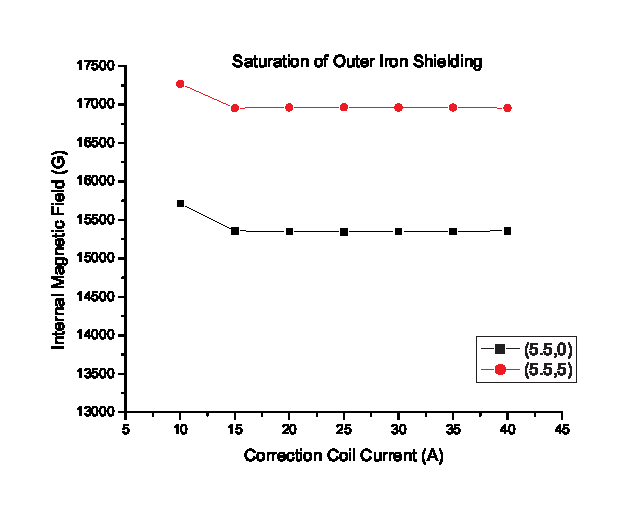
\includegraphics[width=7cm]{R2083_Tapered_0.3cmMiddle_Outer_Shielding_Region.eps}\label{Tapered_Shield_0.3cm_Outer_Region}}
\qquad
\subfloat[Middle Shield Region]
	{\includegraphics[width=7cm]{R2083_Tapered_0.3cmMiddle_Middle_Shielding_Region.eps}\label{Tapered_Shield_0.3cm_Middle_Region}}
\qquad
\subfloat[Inner Shield Region]
	{\includegraphics[width=7cm]{R2083_Tapered_0.3cmMiddle_Inner_Shielding_Region.eps}\label{Tapered_Shield_0.3cm_Inner_Region}}
\caption{\small{Magnetic fields in the R2083 PMT and shield regions using a tapered shield design, consisting of iron-hiperm49-CONETIC layers at a constant 1000 G external field and varying correction coil currents. The outermost layer of iron begins at 1.0~cm thick and slowly thickens to 1.7~cm. The middle layer of hiperm49 is now thinner, at a constant 0.3~cm thick. As seen here, the internal magnetic field is well below the 0.1 G tolerance for the R2083 when the correction coil current is $\approx$25 A. Additionally, the magnetic flux density within the PMT region is much more uniform than previously observed.}}\label{Tapered_Shield_0.3cm}
\end{figure}


%\subsection{Proposed Changes to the Downstream PMT Configuration for use with the R2083}
 
                                                                                                                                                    
Given the restrictions from the current CTOF counter design in Section-\ref{R2083_Triple_No_Coil}, 
the best possible configuration for the triple shield design is an outer shield of NETIC at 1.5~cm thick,
 a middle shield of hiperm49 at 0.8~cm thick, and an inner most layer of CONETIC whose 
thickness is fixed at 0.08~cm by the manufacturer. As seen in Fig.~\ref{R2083_Triple_0.8cm_PMT_Region}
 and with the saturation curves shown in Fig.~\ref{R2083_Triple_0.8cm_Outer}, Fig.~\ref{R2083_Triple_0.8cm_Middle},
 and Fig.~\ref{R2083_Triple_0.8cm_Inner}, the triple shield design with the restrictions imposed by the
 manufacturer and the CTOF counter design specifications will not be effective enough to satisfy the stringent
 0.1~G tolerance required by the R2083.










%\begin{figure}[htbp]%#1
%\begin{center}
%\includegraphics[width=16cm,clip=true,bb=  100 100 500 500]{}
%\end{center}
%\caption{ Magnetisation curve of the shield Netic-Hyperm-Conetic}
%\label{}}
%\end{figure}
%\clearpage
%\newpage


%\begin{figure}[htbp]%#1
%\begin{center}
%\includegraphics[width=16cm,clip=true,bb=  100 100 500 500]{}
%\end{center}
%\caption{ Magnetisation curve of the shield Steel-Hyperm-Conetic}
%\label{}}
%\end{figure}
%\clearpage
%\newpage



%\begin{figure}[htbp]%#1
%\begin{center}
%\includegraphics[width=16cm,clip=true,bb=  100 100 500 500]{}
%\end{center}
%\caption{Magnetisation curve of the shield Steel-conetic-conetic }
%\label{FEAR2083saclay3}}
%\end{figure}
%\clearpage
%\newpage






\section{Conclusion and outlook}




%Given the restrictions from the current CTOF counter design, 
%the triple shield design with an outer shield of iron at 1.7~cm thick,
% a middle shield of hiperm49 at 0.3~cm thick, and an inner most layer of CONETIC whose 
%thickness is fixed at 0.08~cm by the manufacturer.
The triple shield design with the restrictions imposed by the
 manufacturer and the CTOF  specifications will  be effective  to 
satisfy the stringent 0.4~G tolerance only.
To further reduce the magnetic field within acceptable tolerances, a novelle 
hybrid magnetic shielding was developed
using a correction coil and a tapered outer shield of iron. 
%From Fig.~\ref{Tapered_Shield_0.3cm_PMT_Region},
 It has been shown that it is possible to reduce the internal magnetic field to far  below 0.1 G, permitting the
 R2083 to operate with high timing resolution.



\end{document}










\section{12345Measurements with the prototype of teh Hybrid Magnetic Shield for R2083.}

The inner field strongly
depends on the ferromagnetic properties which are very sensible to
fabrication technologies.
\subsection{Hyperm 49 with compensating coil}
\subsection{Big shield with compensating coil}

\subsection{Soft Iron shield for R2083 from Hamamatsu}
\begin{figure}[htbp]
\centering
\includegraphics[width=1\textwidth]{soft_iron_r2083.eps}
\caption{\small{Performance of the soft iron shield for the CTOF under 0 to 75G external field}}
\label{R2083_Soft_Iron}
\end{figure}
\subsection{Thick soft iron without coil}





%>>>>>>> 1.10





\begin{figure}[htbp]%#1
\begin{center}
\includegraphics[width=16cm,clip=true,bb=  100 100 500 500]{}
\end{center}
\caption{Magnetisation curve of the  Steel shield.}
\label{FEAR2083saclay3}}
\end{figure}
\clearpage
\newpage




\begin{figure}[htbp]%#1
\begin{center}
\includegraphics[width=16cm,clip=true,bb=  100 100 500 500]{}
\end{center}
\caption{Magnetisation curve of the  Netic shield.}
\label{FEAR2083saclay3}}
\end{figure}
\clearpage
\newpage



\begin{figure}[htbp]%#1
\begin{center}
\includegraphics[width=16cm,clip=true,bb=  100 100 500 500]{}
\end{center}
\caption{Shield effectiveness vs the length of the shield.}
\label{FEAR2083saclay3}}
\end{figure}
\clearpage
\newpage


%%%%%%%%%%%%%%%%%%%%%%%%%%%%%%%%%%%%%%%%%%%%%%%%%%%%%%%%%%%%%%%%%%%%%THEEND%%%%%%%%%%%%%%%%%%%%%%%%%%%










\subsection{H8500 Shield in homogeneous magnetic field 3000 G}

\begin{table}[htbp]
\begin{center}
\begin{tabular}{|c|c|c|c|c|c|c|c|c|c|} \hline
Cyl&$B_{o}       $ & $D_+$ &  $D_-$ & $t$    &  $B_m$ & $\approx\mu$ &  $S$  & $B_{in}$          & Comm. \\  &      $G$     & $mm$  &  $mm$  & $mm$   &   $G$ &              &       & $G$              &       \\ \hline
1& 50              & 164.75& 158.75(6.25'') &   3.175(0.125'')    &  2578  &   4500       & 110   &  0.46             & Net
%1& 50              & 164.75& 156.75 &   4    &  2578  &   4500       & 110   &  0.46             & Netic \\ \hline
2& 0.46            & 153.41 & 151.37  &  1.02(0.04'')   &  2185  &   400000     & 530   &  0.001            & Netic
%2& 0.46            & 151.37& 149.77 &  0.4   &  2185  &   400000     & 530   &  0.001            & Conetic      \\
%3& 0.001           & 144.0 &  142.4 &  0.76   &   3185 &  450000      & 11000 &  0.007            &       \\ \hline
3& 0.001            & 144.0 &  142.4 &  0.51(0.02'')   &   3185 &  450000      & 11000 &  0.007
\end{tabular}
\end{center}
\caption{HTCC  shield  against of  $50G$. \label{htcc}}
\end{tablemu250}
%\end{document}




\begin{table}[htbp]
\begin{center}
\begin{tabular}{|c|c|c|c|c|c|c|c|c|c|} \hline
Cyl&$B_{o}       $ & $D_+$ &  $D_-$ & $t$    &  $B_m$ & $\approx\mu$ &  $S$  & $B_{in}$          & Comm. \\  &      $G$     & $mm$  &  $mm$  & $mm$   &   $G$ &              &       & $G$              &       \\ \hline
1& 2000              & 106& 74 &  16  & 16600  & 1600  & 241   &  8.3        & Netic
1& 2000              & 106& 74 &  16  & 16600  & 160   & 24    &  83         & Carp BF \\ \hline
2&  17               &  74& 70 &  1.6 &   982  & 1-2e3 & 20-40 & 0.4-0.8     & Netic x 0.01 conetic
2&  160              &  74& 70 &  1.6 &  7400  & 1-2e5 & 2-4e3 & 0.04-0.08   & Hyperm-49
%2& 0.46            & 151.37& 149.77 &  0.4   &  2185  &   400000     & 530   &  0.001            & Conetic      \\
%3& 0.001           & 144.0 &  142.4 &  0.76   &   3185 &  450000      & 11000 &  0.007            &       \\ \hline
3& 0.001            & 144.0 &  142.4 &  0.51(0.02'')   &   3185 &  450000      & 11000 &  0.007
\end{tabular}
\end{center}
\caption{R2083  shield  against of  $2000G$. Comparison of the  Carpenter and Netic alloys.
Conetic is 10 times more efficient at 16600 G field inside the material. Therfore it is safer to use
Netic as a first layer. The second layer may be Co-netic  even 0.8mm thick
 \label{htcc}}
\end{tablemu250}
%\end{document}









\begin{table}[htbp]
\begin{center}
\begin{tabular}{|c|c|c|c|c|c|c|c|c|c|} \hline
Cyl&$B_{o}$ &$D_+$  &$D_-$   & $t$   &  $B_m$ &$\approx\mu$&  $S$  & $B_{in}$          & Comm. \\
   & $G$   &$mm$   &$mm$    & $mm$  &   $G$ &            &       & $G$              &       \\ \hline
1& 700      & 102   & 88    & 6.6    & 13000   &     2600  & 168   &  4.2         & CaB-FM     \\
1& 1000     & 106   & 74     & 8     & 16500  &      160   &  12   &  83          & CaB-FM     \\ \hline
2& 160      &  74   & 70     & 1.6   &   9250 &      5000  & 125   & 1.28         & Netic      \\
2& 160      &  74   & 70     & 1.6   &   9250 &      6200  &  147  & 1.13         & CaB-FM     \\ \hline
3& 3        &  67.2 & 64     & 0.8   &   350  &      44000 & 520   & 0.006        & hyperm-49  \\ \hline
3& 10       &  67.2 & 64     & 0.8   &   1062 &      65000 & 735   & 0.014        & hyperm-49  \\ \hline
3& 20       &  67.2 & 64     & 0.8   &   2120 &     100000 & 1130  & 0.018        & hyperm-49  \\ \hline
3& 30       &  67.2 & 64     & 0.8   &   3200 &     150000 & 1600  & 0.018        & hyperm-49  \\ \hline
3& 40       &  67.2 & 64     & 0.8   &   4250 &     180000 & 2080  & 0.019        & hyperm-49  \\ \hline
3& 50       &  67.2 & 64     & 0.8   &   5300 &     260000 & 3120  & 0.016        & hyperm-49  \\ \hline
3& 70       &  67.2 & 64     & 0.8   &   7400 &     220000 & 2500  & 0.027        & hyperm-49  \\ \hline
3& 80       &  67.2 & 64     & 0.8   &   8500 &     170000 & 2000  & 0.04        & hyperm-49  \\ \hline
3& 90       &  67.2 & 64     & 0.8   &   9600 &      96000 & 1130  & 0.08        & hyperm-49  \\ \hline
3& 100      &  67.2 & 64     & 0.8   &  10620 &      35000 & 411   & 0.24          & hyperm-49  \\ \hline
\end{tabular}
\end{center}
\caption{R2083  shield from Tom Bayley   against of  $1000G$.
Comparison of the  Carpenter and Netic alloys.
Conetic is 10  times more efficient at 100 Oe field inside the material. Therefore it is safer to use
Netic as a first layer. However, 10-15% increas in  material thickness makes it possible to use , for instance,
Carpenter Silicon Core Iron B-FM, the magnetisation curve of which is lower of that for Netic at $H\ge5-7 Oe$.
The second layer may be Hiperm-49 1.6 mm or  even Co-netic   0.8mm thick
 \label{htcc}}
\end{tablemu250}
%\end{document}































%%%%%%%%%%%%%%%%%%%%%%%%%%%%%%
\begin{table}[htbp]
\begin{center}
\begin{tabular}{|c|c|c|c|c|c|c|c|c|c|} \hline
Cyl&$B_{o}       $ & $D_+$ & $D_-$ & $t$    &  $B_m$ & $\approx\mu$ &  $S$  & $B_{in}$          & Comm. \\
\# &      $G$     & $mm$  & $mm$  & $mm$   &   $G$ &              &       & $G$              &       \\ \hline
1& 3000            & 105   &  66   &  19.8  &  20000 &     250      &  47.1 &  63.7             & Netic \\ \hline
%2& 63.7            &  64   &  63.4 &  0.8   &   6370 &   80000      &  1000 &  0.064            & Conetic      \\
%2& 63.7            &  64   &  60.8 &  1.6   &   3185 &  450000      & 11000 &  0.007            & Conetic      \\ \hline
2& 63.7            &  64   &  63.4 &  1.6   &   3185 &    4500      &  110  &  0.7              & Netic       \\
%3& 0.064           &  60   &  58.4 &  0.8   &     6  & 60000        &   800 &      0            & E989-05      \\ \hline
3& 0.7             &  60   &  58.4 &  0.8   &    60  &      80000   &   1000 & 0.7\times10^{-3} & E989-05      \\ \hlin
\end{tabular}
\end{center}
\caption{R2083 shield   against of  $3000G$ at   ferromagnetic  $B_m=20000G$  and corresponding $\mu(B_m)=250$.
 $n$
-layer number starting from the external layer,
 $B_{o}$
-external field,
$D_+$
-external diameter,
$t$
-ferromagnetic thickness,
$B_m$
 -fields in the ferromagnetic determined via Eq.\ref{eq000},
$\mu$
-permeability determined via Fig.\ref{muneco},
$S$
-shielding factor  determined via Eq.\ref{eq000} ,
$B_{in}$
-fields inside the shielding.
$Fm$
-ferromagnetic material.
\label{ca20000}}
\end{tablemu250}
%\end{document}




\begin{table}[htbp]
\begin{center}
\begin{tabular}{|c|c|c|c|c|c|c|c|c|c|} \hline
Cyl&$B_{o}       $ & $D_+$ & $D_-$ & $t$    &  $B_m$ & $\approx\mu$ &  $S$  & $B_{in}$          & Comm. \\
\# &      $G$     & $mm$  & $mm$  & $mm$   &   $G$ &              &       & $G$              &       \\ \hline
1& 3000            & 115   &  66   &  24.5  &  17600 &   1000       &  213  &  63.7             & Netic \\ \hline
2& 63.7            &  64   &  63.4 &  0.8   &   6370 &   80000      &  1000 &  0.064            & Conetic      \\
2& 63.7            &  64   &  60.8 &  1.6   &   3185 &  450000      & 11000 &  0.007            & Conetic      \\ \hline
3& 0.064           &  60   &  58.4 &  0.8   &     6  & 60000        &   800 &      0            & E989-05      \\ \hline
\end{tabular}
\end{center}
\caption{R2083  shield  against of  $3000G$ at  maximum ferromagnetic   $B_m=17600 G$ and
 $\mu(B_m)\approx 1000$. \\
$B_{o}$ - external field(s) for the \#'s-layer  \\
$t$   - the ferromagnetic thickness,  determined via  Eq.\ref{eq000})  \\
$\mu$ - permeability, determined from Fig.\ref{muneco} \\
$B_{in}$ -fields inside the  shielding cylinder .\\
The external shield diameter $115mm$
\label{ca17600}}
\end{tablemu250}
%\end{document}



\begin{table}[htbp]
\begin{center}
\begin{tabular}{|c|c|c|c|c|c|c|c|c|c|} \hline
Cyl&$B_{o}       $ & $D_+$ &  $D_-$ & $t$    &  $B_m$ & $\approx\mu$ &  $S$  & $B_{in}$          & Comm. \\
\# &      $G$     & $mm$  &  $mm$  & $mm$   &   $G$ &              &       & $G$              &       \\ \hline

1& 50              & 164.75& 158.75(6.25'') &   3.175(0.125'')    &  2578  &   4500       & 110   &  0.46             & Net
%1& 50              & 164.75& 156.75 &   4    &  2578  &   4500       & 110   &  0.46             & Netic \\ \hline
2& 0.46            & 153.41 & 151.37  &  1.02(0.04'')   &  2185  &   400000     & 530   &  0.001            & Netic
%2& 0.46            & 151.37& 149.77 &  0.4   &  2185  &   400000     & 530   &  0.001            & Conetic      \\
%3& 0.001           & 144.0 &  142.4 &  0.76   &   3185 &  450000      & 11000 &  0.007            &       \\ \hline
3& 0.001            & 144.0 &  142.4 &  0.51(0.02'')   &   3185 &  450000      & 11000 &  0.007
\end{tabular}
\end{center}
\caption{HTCC  shield  against of  $50G$.
$B_{o}$ - external field(s) for the \#'s-layer  \\
$t$   - the ferromagnetic thickness,  determined via  Eq.\ref{eq000})  \\
$\mu$ - permeability, determined from Fig.\ref{muneco} \\
$B_{in}$ -fields inside the  shielding cylinder .\\
The external shield diameter $115mm$
\label{ca17600}}
\end{tablemu250}


\end{document}

























\newpage
\section{Further  possible studies with micro channel PMTs}


\paragraph{Motivation} manufacturers($Burle$) of the micro channel
plate PMTs are making progress
          in the design of the MCP PMs. This may result in higher
          counting rate and higher magnetic field immunity, as well.
          $Burle$ is developing 10- an 5-micron MCP PMs such as 18mm 85104
	  with increased QE of $20-30\%$ .
\begin{enumerate}

     \item
Develop a setup of 2 10(5) micron MCP PMs with on board
          pre-amplifiers.

     \item
perform resolution/counting rate  tests with 2 MCP PMTs
\end{enumerate}

\paragraph{Current status} preliminary publications are done
                and  preliminary discussions  with the detector group members.
We plan  to  publish  in NIM our recent results obtained with Burle
          85011 PMs. This paper will include the description of the
          on-board preamplifier, resolution measurements and, perhaps ,
          magnetic field tests performed by the detector group.

\paragraph{Labor}     $40 man\times day$ for  Pre-Amp/HV dividers by the
Detector Group.
\paragraph{Equipment} Electronic lab of JLAB for  Pre-Amp/HV dividers.
\paragraph{Materials} 2 MCP  PMTs, HV components  for voltage dividers.
\paragraph{Funding}   8000\$(from Detector Group?) for 2 MCP  PMTs and electronics
components
<<<<<<< ctofmagshield310108.tex



\newpage
\end{document}


%%%%%%%
%%%%%%%%
%%%%%%%%%
%%%%%%%%%%
%%%%%%%%%%%
%%%%%%%%%%%






\subsection{Magnetic Shield for the XP4508B Photomultiplier Tube}

%(Travis insert writeup here)
A magnetic shielding model was developed and theoretically 
tested for the 5 inchXP 4508B Photomultiplier tube.  
The program Poisson Superfish was used to examine the shielding properties of
various shield setups subject to an external magnetic field up to 60 Gauss.  
The sensitivity of the PMT requires a very low (~.2 Gauss) 
magnetic field at the location of the photocathode.

\subsubsection{Single Layer Shielding}

The first shield design tested was a single 1.6mm 
thick shield surrounding the PMT with an inner radius of 7.657cm. 
 An external magnetic field was applied to the shielded area ranging from
0 to 60 Gauss.  The calculated magnetic field strength was recorded
 at critical points (the center of the shielded area, location of the
 photocathode, close to the inner radius of the shield,
and inside the shield).  The calculations were performed with 2 different
 materials, conetic and hyperm49.  The ferromagnetic properties of these materials
were well known, so we wanted to see how well they would perform in our 
particular configuration.  Experimental data was also collected for this 
size shielding made of a $50\%$ alloy of NiFe
and was compared to our theoretical calculations.  The graph below shows
 the strength of the magnetic field at the center of the shield for the 
different materials listed.

\newpage
\begin{figure}[htbp]
\centering
\includegraphics[width=.6\textwidth]{SS_Materials.eps}
\caption{\small{Single Shield Material Comparison}}
\label{Single mu-metal shield 1.6mm thick 76mm in radius.}
\end{figure}



None of these 3 shields performed adequately enough to limit the strength of 
the magnetic field to less than 0.1 Gauss when an external field of around 50 G
 was applied, so we explored the effect of increasing the thickness of the shield.  
Calculations were performed for a single 3.2mm thick shield with the same inner
 radius of 7.657cm with 4 materials: regular iron, netic (soft iron),conetic, 
and hyperm49.  Increasing the thickness of the shield clearly helped to provide
 better shielding from the external field, but not by a significant enough
 amount to achieve the desired field of 0.1 Gauss.  This led us to conclude 
a single layer shield would be insufficient for our design, so we began to
 test 2 layer shielding models; however, we were able to determine that 
hyperm49 and conetic performed much better than 
netic or iron, with hyperm49 
seemingly the best for our purposes.

\begin{figure}[htbp]
\centering
\includegraphics[width=.6\textwidth]{SS_32.eps}
\caption{\small{Magnetic Field at location of Photocathode}}
\label{Single Shield 3.2mm Thick}
\end{figure}


\subsubsection{2 Layer Shielding}

Four   configurations were tested for 2 layer shields with fixed
 inner diameters of 5.795 and 6.135 inches for the inner and outer 
shields, respectively.  The inner shield was made of conetic and was
 either 1.0mm or 1.6mm thick, while the outer shield was made of netic 
(soft iron) and was either 4.0mm or 6.0mm thick.  The strength of the
 magnetic field was again calculated and recorded at the location of
 the photocathode, shown below.  The varying thicknesses made very little 
difference in the calculated magnetic field strength (less than 0.1 G),
 but the setup with the maximum thicknesses (netic at 6.0mm, conetic 1.6mm)
 was slightly better than the others.  The measured magnetic field at H=50
 Gauss was still 0.79G, which is still far too high for the PMT to operate correctly.

\begin{figure}[htbp]
\centering
\includegraphics[width=.6\textwidth]{DS.eps}
\caption{\small{Magnetic Field at location of Photocathode}}
\label{Double Layer Shield}
\end{figure}

\subsubsection{3 Layer Shielding}

For these calculations a 3rd shield was introduced, 
the shield manufactured by Photonis that was distributed
 with the PMT.  This shield is made of Mu-Metal MS175, but
 we approximated this material with our known magnetic
 permeability for the Mu-Metal conetic.  The outer 2 shields were
 the exact same as in the 2 layer model described above, so we
 merely repeated the same calculations with the addition of this 
third inner shield of conetic.  The addition of this third shield
 helped somewhat, but not to the degree required to reduce the
 field to 0.1 or 0.2 Gauss.  The recorded field at the location
 of the photocathode was still about 0.6 Gauss with a 6mm netic
 outer shield and 1.6mm conetic middle shield.

\newpage
\begin{figure}[htbp]
\centering
\includegraphics[width=.6\textwidth]{TS.eps}
\caption{\small{Magnetic Field at location of Photocathode}}
\label{Triple Layer Shield}
\end{figure}

From our 1 layer shielding calculations,
 it was clear that hyperm49 would provide better
 shielding than netic, so we modified the 3 layer model
 above by switching the material of the outer shield from 
netic to hyperm49.  Since the best 3 layer shield was with
 a 6mm thick layer of netic and a 1.6mm thick layer of conetic,
 we used these sizes for this model as well, with a 6mm thick
 layer of hyperm49, a 1.6mm thick layer of conetic, and the inner
 Photonis shield of conetic.  This simple alteration helped to 
improve the shielding of the model significantly, reducing the magnetic
 field strength at the photocathode from 0.69 to 0.28 at an external
 field strength of 50G.  The field strength at an external field of 35G 
(which is the expected field strength) is about 0.2G, which is close to
 the required level for correct operation of the PMT.

\begin{figure}[htbp]
\centering
\includegraphics[width=.6\textwidth]{TS_Compare.eps}
\caption{\small{Magnetic Field at location of Photocathode}}
\label{Triple Layer Shield Comparison}
\end{figure}

\subsubsection{Conclusion}

From the variety of calculations performed, it is clear that a
 3 layer shielding model using the materials Hyperm49 and conetic
 would provide the best shielding from external fields up to 60 Gauss.  
The best model tested was an outer shield of Hyperm49 with 6mm thickness
 and 6.135 inch inner diameter, a middle shield of conetic with 1.6mm 
thickness and 5.795 inch inner diameter, and the inner Photonis Mu-metal
 shield with inner diameter 5.500 inches.  
This model would reduce an
 external field of ~35G to ~0.2G at the location of the photocathode. 
 Further improvements on this shielding model might involve a thicker
 outer shield of hyperm49, lengthening of shields (in the axial direction)
 to extend farther from the photocathode, or replacing the Photonis inner
 shield with one of different size.  The materials hyperm49 and conetic
 perform nearly identically up to about a 50G external field (at which 
point hyperm49 becomes far superior), so interchanging conetic and hyperm49
 on the inner shields would probably not have a significant effect on the
 strength of the magnetic field.




From this section we conclude that in order to achieve the fields below 0.2G
we havew to develop some new solutions. One of such solutions is 
described in the following section.

%%%%%%%%%%%%%%%%%%%%
\section{Magnetic Shield for the XP4508B Photomultiplier Tube}

A magnetic shielding model was developed and theoretically tested for the 5 inch XP4508B Photomultiplier tube.  The program Poisson Superfish was used to examine the shielding properties of 
various shield setups subject to an external magnetic field up to 60 Gauss.  The sensitivity of the PMT requires a very low (~.2 Gauss) magnetic field at the location of the photocathode.

\subsection{Single Layer Shielding}

The first shield design tested was a single 1.6mm thick shield surrounding the PMT with an inner radius of 7.657cm.  An external magnetic field was applied to the shielded area ranging from
0 to 60 Gauss.  The calculated magnetic field strength was recorded at critical points (the center of the shielded area, location of the photocathode, close to the inner radius of the shield,
and inside the shield).  The calculations were performed with 2 different materials, conetic and hyperm49.  The ferromagnetic properties of these materials 
were all well known, so we wanted to see how well they would perform in our particular configuration.  Experimental data was also collected for this size shielding made of a 50% alloy of NiFe
and was compared to our theoretical calculations.  The graph below shows the strength of the magnetic field at the center of the shield for the different materials listed.

%\begin{figure}[htbp]
%\centering
%\includegraphics[width=.6\textwidth]{/madlem/data/SS_Materials.eps}
%\caption{\small{Single Shield Material Comparison}}
%\label{Single Shield Material Comparison}
%\end{figure}



None of these 3 shields performed adequately enough to limit the strength of the magnetic field to less than 0.1 Gauss when an external field of around 50 G was applied, so we explored the effect of increasing the thickness of the shield.  Calculations were performed for a single 3.2mm thick shield with the same inner radius of 7.657cm with 4 materials: regular iron, netic (soft iron),conetic, and hyperm49.  Increasing the thickness of the shield clearly helped to provide better shielding from the external field, but not by a significant enough amount to achieve the desired field of 0.1 Gauss.  This led us to conclude a single layer shield would be insufficient for our design, so we began to test 2 layer shielding models; however, we were able to determine that hyperm49 and conetic performed much better than netic or iron, with hyperm49 seemingly the best for our purposes.

%\begin{figure}[htbp]
%\centering
%\includegraphics[width=.6\textwidth]{/madlem/data/SS_32.eps}
%\caption{\small{Magnetic Field at location of Photocathode}}
%\label{Single Shield 3.2mm}
%\end{figure}


\subsection{2 Layer Shielding}

As directed by my mentor, I tested 4 different configurations for 2 layer shields with fixed inner diameters of 5.795 and 6.135 inches for the inner and outer shields, respectively.  The inner shield was made of conetic and was either 1.0mm or 1.6mm thick, while the outer shield was made of netic (soft iron) and was either 4.0mm or 6.0mm thick.  The strength of the magnetic field was again calculated and recorded at the location of the photocathode, shown below.  The varying thicknesses made very little difference in the calculated magnetic field strength (less than 0.1 G), but the setup with the maximum thicknesses (netic at 6.0mm, conetic 1.6mm) was slightly better than the others.  The measured magnetic field at H=50 Gauss was still 0.79G, which is still far too high for the PMT to operate correctly.

%\begin{figure}[htbp]
%\centering
%\includegraphics[width=.6\textwidth]{/madlem/data/DS.eps}
%\caption{\small{Magnetic Field at location of Photocathode}}
%\label{Double Layer Shield}
%\end{figure}

\subsection{3 Layer Shielding}

For these calculations a 3rd shield was introduced, the shield manufactured by Photonis that was distributed with the PMT.  This shield is made of Mu-Metal MS175, but we approximated this material with our known magnetic permeability for the Mu-Metal conetic.  The outer 2 shields were the exact same as in the 2 layer model described above, so we merely repeated the same calculations with the addition of this third inner shield of conetic.  The addition of this third shield helped somewhat, but not to the degree required to reduce the field to 0.1 or 0.2 Gauss.  The recorded field at the location of the photocathode was still about 0.6 Gauss with a 6mm netic outer shield and 1.6mm conetic middle shield.

%\begin{figure}[htbp]
%\centering
%\includegraphics[width=.6\textwidth]{/madlem/data/TS.eps}
%\caption{\small{Magnetic Field at location of Photocathode}}
%\label{Triple Layer Shield}
%\end{figure

From our 1 layer shielding calculations, it was clear that hyperm49 would provide better shielding than netic, so we modified the 3 layer model above by switching the material of the outer shield from netic to hyperm49.  Since the best 3 layer shield was with a 6mm thick layer of netic and a 1.6mm thick layer of conetic, we used these sizes for this model as well, with a 6mm thick layer of hyperm49, a 1.6mm thick layer of conetic, and the inner Photonis shield of conetic.  This simple alteration helped to improve the shielding of the model significantly, reducing the magnetic field strength at the photocathode from 0.69 to 0.28 at an external field strength of 50G.  The field strength at an external field of 35G (which is the expected field strength) is about 0.2G, which is close to the required level for correct operation of the PMT.

%\begin{figure}[htbp]
%\centering
%\includegraphics[width=.6\textwidth]{/madlem/data/TS_Compare.eps}
%\caption{\small{Magnetic Field at location of Photocathode}}
%\label{Triple Layer Shield Comparison}
%\end{figure

\subsection{Conclusion}

From the variety of calculations performed, it is clear that a 3 layer shielding model using the materials Hyperm49 and conetic would provide the best shielding from external fields up to 60 Gauss.  The best model tested was an outer shield of Hyperm49 with 6mm thickness and 6.135 inch inner diameter, a middle shield of conetic with 1.6mm thickness and 5.795 inch inner diameter, and the inner Photonis Mu-metal shield with inner diameter 5.500 inches.  This model would reduce an external field of ~35G to ~0.2G at the location of the photocathode.  Further improvements on this shielding model might involve a thicker outer shield of hyperm49, lengthening of shields (in the axial direction) to extend farther from the photocathode, or replacing the Photonis inner shield with one of different size.  The materials hyperm49 and conetic perform nearly identically up to about a 50G external field (at which point hyperm49 becomes far superior), so interchanging conetic and hyperm49 on the inner shields would probably not have a significant effect on the strength of the magnetic field.


\subsection{Hybrid Magnetic Shielding with R2083}

In conjunction with the triple shield model from Fig.~\ref{R2083_Initial}, 
it has been proposed that the use of a correction coil placed between two layers
 of shielding should decrease the magnetic field to below the 0.1~G threshold required 
by the R2083. In all tests involving a correction coil,
 the external magnetic field was kept at a constant 1000~G.

\subsubsection{Effect of Correction Coil}

The initial shield design shown in Fig.~\ref{R2083_Initial} was reconfigured such that the 
middle shielding layer of hiperm49 was increased to 0.5~cm thick, 
and the outer layer of NETIC is 1.0~cm thick. 
This was done to reduce the weight and cost of the materials. The new design with the correction coil
 between the CONETIC and hiperm49 layer is shown 
in Fig.~\ref{R2083CorrectionCoilStandardDesign.eps}.
%
\begin{figure}[htbp]
\centering
\includegraphics[width=1.0\textwidth]{R2083CorrectionCoilStandardDesign.eps}
\caption{\small{The  shield with correction coil. 
The external magnetic field is set at 1000 G.  The field map  is shown when the correction coil is set to 25 A.}}
\label{R2083_Correction_Coil}
\end{figure}
%
In order to understand the behavior of the internal magnetic field as it approached 0~G,
 the sign of the z-component of the magnetic field was used in conjunction with the 
absolute magnitude of the total magnetic field. 
As seen in Fig.~\ref{R2083_Correction_Coil_PMT_Region}, the utilization of the correction coil is capable of reducing the internal magnetic field to within acceptable tolerances, but this design requires further optimization.

\begin{figure}[ht]
\centering
\subfloat[PMT Region]
	{\includegraphics[width=7cm]{R2083_Correction_Coil_PMT_Region.eps}\label{R2083_Correction_Coil_PMT_Region}}
\qquad
\subfloat[Outer Shield Region]
{\includegraphics[width=7cm]{R2083_Correction_Coil_Outer_Region.eps}\label{R2083_Correction_Coil_Outer_Region}}
\qquad
\subfloat[Middle Shield Region]
{\includegraphics[width=7cm]{R2083_Correction_Coil_Middle_Region.eps}\label{R2083_Correction_Coil_Middle_Region}}
\qquad
\subfloat[Inner Shield Region]
{\includegraphics[width=7cm]{R2083_Correction_Coil_Inner_Region.eps}\label{R2083_Correction_Coil_Inner_Region}}
\caption{\small{Effect of changing current of the correction coil on internal magnetic field strength within the PMT and shield regions. The external magnetic field is kept constant at 1000 Gauss.}}\label{R2083_Correction_Coil2}
\end{figure}
\clearpage
\newpage

